\documentclass[twoside]{book}

% Packages required by doxygen
\usepackage{fixltx2e}
\usepackage{calc}
\usepackage{doxygen}
\usepackage[export]{adjustbox} % also loads graphicx
\usepackage{graphicx}
\usepackage[utf8]{inputenc}
\usepackage{makeidx}
\usepackage{multicol}
\usepackage{multirow}
\PassOptionsToPackage{warn}{textcomp}
\usepackage{textcomp}
\usepackage[nointegrals]{wasysym}
\usepackage[table]{xcolor}

% Font selection
\usepackage[T1]{fontenc}
\usepackage[scaled=.90]{helvet}
\usepackage{courier}
\usepackage{amssymb}
\usepackage{sectsty}
\renewcommand{\familydefault}{\sfdefault}
\allsectionsfont{%
  \fontseries{bc}\selectfont%
  \color{darkgray}%
}
\renewcommand{\DoxyLabelFont}{%
  \fontseries{bc}\selectfont%
  \color{darkgray}%
}
\newcommand{\+}{\discretionary{\mbox{\scriptsize$\hookleftarrow$}}{}{}}

% Page & text layout
\usepackage{geometry}
\geometry{%
  a4paper,%
  top=2.5cm,%
  bottom=2.5cm,%
  left=2.5cm,%
  right=2.5cm%
}
\tolerance=750
\hfuzz=15pt
\hbadness=750
\setlength{\emergencystretch}{15pt}
\setlength{\parindent}{0cm}
\setlength{\parskip}{3ex plus 2ex minus 2ex}
\makeatletter
\renewcommand{\paragraph}{%
  \@startsection{paragraph}{4}{0ex}{-1.0ex}{1.0ex}{%
    \normalfont\normalsize\bfseries\SS@parafont%
  }%
}
\renewcommand{\subparagraph}{%
  \@startsection{subparagraph}{5}{0ex}{-1.0ex}{1.0ex}{%
    \normalfont\normalsize\bfseries\SS@subparafont%
  }%
}
\makeatother

% Headers & footers
\usepackage{fancyhdr}
\pagestyle{fancyplain}
\fancyhead[LE]{\fancyplain{}{\bfseries\thepage}}
\fancyhead[CE]{\fancyplain{}{}}
\fancyhead[RE]{\fancyplain{}{\bfseries\leftmark}}
\fancyhead[LO]{\fancyplain{}{\bfseries\rightmark}}
\fancyhead[CO]{\fancyplain{}{}}
\fancyhead[RO]{\fancyplain{}{\bfseries\thepage}}
\fancyfoot[LE]{\fancyplain{}{}}
\fancyfoot[CE]{\fancyplain{}{}}
\fancyfoot[RE]{\fancyplain{}{\bfseries\scriptsize Generated by Doxygen }}
\fancyfoot[LO]{\fancyplain{}{\bfseries\scriptsize Generated by Doxygen }}
\fancyfoot[CO]{\fancyplain{}{}}
\fancyfoot[RO]{\fancyplain{}{}}
\renewcommand{\footrulewidth}{0.4pt}
\renewcommand{\chaptermark}[1]{%
  \markboth{#1}{}%
}
\renewcommand{\sectionmark}[1]{%
  \markright{\thesection\ #1}%
}

% Indices & bibliography
\usepackage{natbib}
\usepackage[titles]{tocloft}
\setcounter{tocdepth}{3}
\setcounter{secnumdepth}{5}
\makeindex

% Hyperlinks (required, but should be loaded last)
\usepackage{ifpdf}
\ifpdf
  \usepackage[pdftex,pagebackref=true]{hyperref}
\else
  \usepackage[ps2pdf,pagebackref=true]{hyperref}
\fi
\hypersetup{%
  colorlinks=true,%
  linkcolor=blue,%
  citecolor=blue,%
  unicode%
}

% Custom commands
\newcommand{\clearemptydoublepage}{%
  \newpage{\pagestyle{empty}\cleardoublepage}%
}

\usepackage{caption}
\captionsetup{labelsep=space,justification=centering,font={bf},singlelinecheck=off,skip=4pt,position=top}

%===== C O N T E N T S =====

\begin{document}

% Titlepage & ToC
\hypersetup{pageanchor=false,
             bookmarksnumbered=true,
             pdfencoding=unicode
            }
\pagenumbering{alph}
\begin{titlepage}
\vspace*{7cm}
\begin{center}%
{\Large ci\+\_\+example\+\_\+cpp }\\
\vspace*{1cm}
{\large Generated by Doxygen 1.8.13}\\
\end{center}
\end{titlepage}
\clearemptydoublepage
\pagenumbering{roman}
\tableofcontents
\clearemptydoublepage
\pagenumbering{arabic}
\hypersetup{pageanchor=true}

%--- Begin generated contents ---
\chapter{ci\+\_\+example\+\_\+cpp}
\label{index}\hypertarget{index}{}\subsection*{What is it}

This package contains a set of examples of demos and unit tests in c++ supported by the continuous integration. It also contains the coding guidelines setup in the \href{https://wp.nyu.edu/machinesinmotion/}{\tt machines-\/in-\/motion} group.

\subsection*{Authors}


\begin{DoxyItemize}
\item Vincent Berenz
\item Maximilien Naveau
\end{DoxyItemize}

\subsection*{Copyrights}

Copyright (c) 2019, New York University and Max Planck Gesellschaft.

\subsection*{License}

License B\+S\+D-\/3-\/\+Clause 
\chapter{2. C++ Coding Guidelines}
\label{coding_guidelines_1}
\Hypertarget{coding_guidelines_1}
\subsection*{I. Introduction}

These are the internal C++ guidelines for the \href{https://wp.nyu.edu/machinesinmotion/}{\tt machines-\/in-\/motion} group. The same guidelines are used in the \href{https://open-dynamic-robot-initiative.github.io/}{\tt Open Dynamic Robot Initiative}

The following rules present basic guidelines for our C++ code. The goal is to have code that is formatted in a consistent and easily readable way while at the same time not being overly complicated by specifying every detail. For such guidelines to be practical, newcomers should be able to read them within a few minutes and be able to memorize them. So these rules intentionally do not cover every detail but rather aim at specifying only the big, important things.

If this is too simple for you and you want more rules, you are encouraged to read the \href{https://google.github.io/styleguide/cppguide.html}{\tt Google C++ Style Guide} on which these rules are based. Note, however, that we have a few small deviations from the Google style.

These guidelines may evolve in time so it is first good practice to check them upon creation of a new package or code refactoring.

\subsection*{II. Folder Structure and File Naming}


\begin{DoxyItemize}
\item Header files should be in a folder\+: {\ttfamily include/$<$name\+\_\+of\+\_\+the\+\_\+project$>$/$\ast$}, e.\+g.
\begin{DoxyCode}
`#include "ci\_example\_cpp/gains\_configuration.hpp"` 
\end{DoxyCode}

\item File extension for header files\+: {\ttfamily .hpp}
\item Source files should be in a folder named {\ttfamily src/}. The file should have the same name as the header with extension {\ttfamily .cpp}.
\item When using templates\+: If you want to separate declaration and definition, put the declaration to a {\ttfamily .hpp} header file as usual and the definition to a file with extension {\ttfamily .hxx} in the same directory (which is included at the bottom of the {\ttfamily .hpp} file).
\item Preferably each class should be in a separate file with name {\itshape class\+\_\+name\+\_\+in\+\_\+lower\+\_\+case}. However, this is not a strict rule, if several smaller classes are logically closely related, they may go to the same file.
\item Executable scripts should be placed in the {\ttfamily scripts/} folder. And should have a C\+Make {\bfseries install rule} that makes them executable upon installation.
\item The C++/pybind11 code for wrapping C++ code to Python must be placed in {\ttfamily srcpy/}
\end{DoxyItemize}

\subsection*{I\+II. Naming}

Give as descriptive a name as possible, within reason. Do not worry about saving horizontal space as it is far more important to make your code immediately understandable by a new reader. Do not use abbreviations that are ambiguous or unfamiliar to readers outside your project, and do not abbreviate by deleting letters within a word. Abbreviations that would be familiar to someone outside your project with relevant domain knowledge are OK. As a rule of thumb, an abbreviation is probably OK if it\textquotesingle{}s listed in Wikipedia.

Formatting of names should be as follows\+:


\begin{DoxyItemize}
\item types (classes, structs, ...)\+: {\itshape First\+Upper\+Camel\+Case}
\item functions, methods\+: {\itshape lower\+\_\+case\+\_\+with\+\_\+underscores}
\item variables\+: {\itshape lower\+\_\+case\+\_\+with\+\_\+underscores}
\item class members\+: {\itshape like\+\_\+variables\+\_\+but\+\_\+with\+\_\+trailing\+\_\+underscore\+\_\+}
\item constants\+: {\itshape U\+P\+P\+E\+R\+\_\+\+C\+A\+S\+E\+\_\+\+W\+I\+T\+H\+\_\+\+U\+N\+D\+E\+R\+S\+C\+O\+R\+ES}
\item global variables\+: Should generally be avoided but if needed, prefix them with g\+\_\+, i.\+e. {\itshape g\+\_\+variable\+\_\+name}.
\end{DoxyItemize}

\subsection*{IV. Add Units to Variable Names}

Variables that hold values of a specific unit should have that unit appended to the name. For example if a variable holds the velocity of a motor in {\itshape krpm} it should be called {\ttfamily velocity\+\_\+krpm} instead of {\ttfamily just velocity}. Some more examples\+:


\begin{DoxyItemize}
\item duration\+\_\+us (use \char`\"{}u\char`\"{} instead of \char`\"{}µ\char`\"{})
\item voltage\+\_\+mV
\item acceleration\+\_\+mps2 ( $ \frac{m}{s^2} $)
\end{DoxyItemize}

\subsection*{V. C/\+C++ Formatting}

\subsubsection*{V.\+1. Line Length}

Limit the length of lines to 80 characters.

This may seem hard to follow sometimes but makes it much easier to view two or even three files next to each other (important during code review or when resolving merge conflicts).

\subsubsection*{V.\+2. Indentation}


\begin{DoxyItemize}
\item Use spaces instead of tabs.
\item 4 spaces per \char`\"{}tab\char`\"{}.
\end{DoxyItemize}

\subsubsection*{V.\+3. Position of braces}


\begin{DoxyItemize}
\item Opening brace always goes to the next line.
\item {\bfseries Always} add braces for single-\/line if/loop/etc.
\end{DoxyItemize}

Example\+:


\begin{DoxyCode}
\textcolor{keyword}{namespace }bar
\{

\textcolor{keyword}{class }Foo
\{
    \textcolor{keywordtype}{void} my\_function(\textcolor{keyword}{const} Foo &foo, \textcolor{keywordtype}{int} *output\_arg)
    \{
        \textcolor{keywordflow}{if} (condition)
        \{
            ...
        \}
        \textcolor{keywordflow}{else} \textcolor{keywordflow}{if} (other\_condition)
        \{
            ...
        \}
        \textcolor{keywordflow}{else}
        \{
            ...
        \}

        \textcolor{keywordflow}{while} (condition)
        \{
            ...
        \}
    \}
\}

\} \textcolor{comment}{// namespace}
\end{DoxyCode}


\subsubsection*{V.\+3. Spaces}

Add single spaces between if/for/etc., the condition and the brace. add spaces around most binary operators. Exception\+: No spaces around {\ttfamily \+:\+:}, {\ttfamily .} and {\ttfamily -\/$>$}. Also no spaces for unary operators ({\ttfamily i++}, {\ttfamily \&x}, {\ttfamily $\ast$x}, ...).

Example\+: 
\begin{DoxyCode}
\textcolor{keywordtype}{int} x = 42;
\textcolor{keywordflow}{for} (\textcolor{keywordtype}{int} i = 0; i < x; i++)
\{
    \textcolor{keywordtype}{int} y = i * x;
    \textcolor{keywordflow}{if} (y == foo.bar->baz)
    \{
        ...
    \}
\}
\end{DoxyCode}


\subsubsection*{V.\+4. Formatting of switch blocks}


\begin{DoxyItemize}
\item See the following example for proper indentation of switch blocks.
\item Always add a default case, even when it is technically not needed.
\begin{DoxyItemize}
\item If the default block is empty, it shall contain a comment to indicate that this is intentional.
\item The default case shall either be the first or the last case, preferably the last.
\end{DoxyItemize}
\item Non-\/empty cases shall be terminated by an unconditional break.
\end{DoxyItemize}


\begin{DoxyCode}
\textcolor{keywordflow}{switch} (x)
\{
    \textcolor{keywordflow}{case} 1:
        \textcolor{comment}{// ...}
        \textcolor{keywordflow}{break};

    \textcolor{keywordflow}{case} 2:
        \textcolor{comment}{// ...}
        \textcolor{keywordflow}{break};

    \textcolor{keywordflow}{case} 3: \textcolor{comment}{// multiple cases for one block are okay}
    \textcolor{keywordflow}{case} 4:
        \textcolor{comment}{// ...}
        \textcolor{keywordflow}{break};

    \textcolor{keywordflow}{case} 5:           \textcolor{comment}{// BAD. A non-empty case without break should not be}
        something();  \textcolor{comment}{// used}
    \textcolor{keywordflow}{case} 6:
        more();
        \textcolor{keywordflow}{break};

    \textcolor{keywordflow}{default}:
        \textcolor{comment}{// no action needed}
        \textcolor{keywordflow}{break};
\}
\end{DoxyCode}


\subsubsection*{V.\+5. Clang-\/\+Format Configuration}

To automatically format your code according to this guidelines, you can use clang-\/format with the configuration \href{https://github.com/machines-in-motion/mpi_cmake_modules/blob/master/python/mpi_cmake_modules/_clang-format}{\tt here}.

\subsection*{VI. C/\+C++ Coding Guidelines}

\subsubsection*{V\+I.\+1. Pass objects by const reference}

In general, non-\/primitive data types should be passed to functions by const reference instead of by value.


\begin{DoxyCode}
\textcolor{keywordtype}{void} foobar(\textcolor{keyword}{const} Foo &foo);  \textcolor{comment}{// good}
\textcolor{keywordtype}{void} foobar(Foo foo);  \textcolor{comment}{// results in copy of `foo`. Only do this if const}
                       \textcolor{comment}{// reference is not possible for some reason.}
\end{DoxyCode}


\#\#\# V\+I.\+2.
\begin{DoxyCode}
*#pragma once* 
\end{DoxyCode}
 vs Include Guards

Prefer
\begin{DoxyCode}
*#pragma once* 
\end{DoxyCode}
 over include guards. 
\begin{DoxyCode}
*#pragma once* 
\end{DoxyCode}
 is not part of the official standard but is widely supported by compilers and much simpler to maintain.

Note that there are some border cases where
\begin{DoxyCode}
*#pragma once* 
\end{DoxyCode}
 is causing issues (e.\+g. on Windows or when having a weird build setup with symlinks or copies of files). In such cases use traditional include guards. Make sure they have unique names by composing them from the package name and the path/name of the file (e.\+g. M\+Y\+\_\+\+P\+A\+C\+K\+A\+G\+E\+\_\+\+P\+A\+T\+H\+\_\+\+T\+O\+\_\+\+F\+I\+L\+E\+\_\+\+F\+I\+L\+E\+N\+A\+M\+E\+\_\+H). Please {\bfseries do not} add underscore as prefix nor suffix beccause this is reserved for the compiler preproccesor variables.

\subsubsection*{V\+I.\+3. Keep scopes small}

Avoid adding anything to the global namespace if possible. This means


\begin{DoxyItemize}
\item Use a namespace when defining extern symbols.
\item Use an anonymous namespace or static for symbols that are only used internally.
\end{DoxyItemize}

Generally define symbols in the smallest possible scope, i.\+e. if a variable is only used inside one loop, define it inside this loop (however, do not consider this to be a very strict rule, deviate from it where it seems reasonable).

\subsubsection*{V\+I.\+4. Use types with explicit sizes}

The header stdint defines primitive types with explicit sizes\+: {\itshape int32\+\_\+t}, {\itshape uint32\+\_\+t}, {\itshape int16\+\_\+t}, ... They should be preferred over the build-\/in types int, unsigned, short, ... To use them add the following include\+: 
\begin{DoxyCode}
\textcolor{preprocessor}{#include <stdint>}
\end{DoxyCode}
 
\chapter{1. General rules applied in the code base}
\label{coding_guidelines_0}
\Hypertarget{coding_guidelines_0}
\subsection*{I. Introduction}

These are general rules independent of the coding language.

\subsection*{II. Catkin Package and Repository Naming}


\begin{DoxyItemize}
\item Name\+: lower\+\_\+cases\+\_\+with\+\_\+underscore.
\item One repository per catkin package.
\item Same name for package and repository.
\end{DoxyItemize}

\subsection*{I\+II. Versioning}

Use semantic versioning when versioning packages. Short summary\+:


\begin{DoxyItemize}
\item Given a version number M\+A\+J\+O\+R.\+M\+I\+N\+O\+R.\+P\+A\+T\+CH, increment the\+:
\item M\+A\+J\+OR version when you make incompatible A\+PI changes,
\item M\+I\+N\+OR version when you add functionality in a backwards-\/compatible manner, and
\item P\+A\+T\+CH version when you make backwards-\/compatible bug fixes.
\end{DoxyItemize}

Regarding formatting of pre-\/releases (alpha, beta, rc, ...) consider P\+E\+P440, especially when versioning Python packages (note that there is no general conflict with semantic versioning, only the format is a bit different).

\subsection*{IV. Contribution Guidelines}

\subsubsection*{I\+V.\+1. Code revision\+:}

To ensure some level of code quality, all modifications have to be reviewed before they can be merged. This is done via merge requests in Git\+Lab (on Git\+Hub it is called pull request but the concept is the same).

The procedure for adding a change is as follows\+:


\begin{DoxyItemize}
\item When creating branches, use your name as a namespace, e.\+g. {\itshape rickdeckard/my\+\_\+branch}. This is to avoid confusion with branches of other people and to indicate who is responsible for that branch. It is not allowed to push branches without such namespace.
\item Test all your changes and update documentation.
\item When finished, create a merge request to the master branch of the main repository.
\item Add one or more of the maintainers as reviewers. The reviewers will review and maybe request changes.
\item Merging is done by the contributor but is only allowed after all reviewers approved. If the merge will affect other people (e.\+g. by breaking the A\+PI), make sure to inform them, e.\+g. via a Mail on an appropriate mailing list. After a merge request is merged, the feature branch shall be deleted.
\end{DoxyItemize}

Never push directly to master or other top-\/level branches. Never force-\/push to any branch that others are using as well. All your development should happen in branches inside your namespace. To keep the number of branches on the repository low, make sure to delete branches that are not needed anymore.

The top-\/level namespace of the repository should only contain a master branch and maybe a few branches for specific versions. Those branches should be protected so that direct pushing is not possible (everything has to go through merge requests).

\subsubsection*{I\+V.\+2. Some rules for the contributors\+:}


\begin{DoxyItemize}
\item To make life easier for the reviewers and to get your changes merged quickly (thus reducing the risk of merge conflicts), try to keep merge requests rather small. This means that, where possible, a bigger task should be split into smaller sub-\/tasks that can be merged one after another instead of putting everything in one huge merge request.
\item When synchronising your feature branch with upstream, you may want to prefer git rebase over git merge to keep the history of you branch clean. However, when there are complicated merge conflicts, it can be much less painful to use merge, which is okay in this case.
\item On your own branches, you can do whatever you want, i.\+e. it is usually okay to force push there (and even necessary when you rebase). However, when applying changes requested by a reviewer, please do not amend or squash them into older commits but add them as new commits. This makes it easier for the reviewer to see what changed.
\item Do not add functional changes and major reformatting in the same commit as this makes review of the functional changes very difficult.
\item Do add unit tests for new features
\item Do create new demos or update existing demos to make it easier how to use the updated A\+PI
\end{DoxyItemize}

\subsubsection*{I\+V.\+3. Some rules for the reviewers\+:}


\begin{DoxyItemize}
\item To make life easier for the contributors, try to provide reviews in a timely manner. The contributor may be blocked in continuing their work while the merge request is under review.
\item When reviewing, check the following things\+:
\begin{DoxyItemize}
\item Is the style guide followed?
\item Are new features/changes properly documented?
\item And of course\+: Do the changes look reasonable and correct?
\end{DoxyItemize}
\item The one who merges should directly delete the feature branch afterwards.
\end{DoxyItemize}

\subsection*{V. Documentation}

\subsubsection*{V.\+1 In-\/code documentation}

All code {\bfseries shall} be documented in-\/source using Doxygen. This means that every function, class, struct, global variable, etc, needs to have a docstring containing some documentation in\+:
\begin{DoxyItemize}
\item \href{https://google.github.io/styleguide/pyguide.html?showone=Comments#Comments}{\tt Google} format for Python,
\item \href{http://www.doxygen.nl/manual/index.html}{\tt Doxygen} format for C/\+C++.
\end{DoxyItemize}

If the definition and declaration are separated (C/\+C++), Doxygen should be in the header, not the cpp file. {\bfseries Please do not duplicate!}.

If you are using catkin, the package should include the mpi\+\_\+cmake\+\_\+modules package and in the C\+Make\+Lists.\+txt file call the {\ttfamily build\+\_\+doxygen\+\_\+documentation()} or the {\ttfamily default\+\_\+mpi\+\_\+cmake\+\_\+modules()}(future) macros. The documentation can then be build via catkin\+\_\+make -\/\+D\+B\+U\+I\+L\+D\+\_\+\+D\+O\+C\+U\+M\+E\+N\+T\+A\+T\+I\+ON=ON.

Make the documentation as compact as possible. Avoid boilerplate formulations that do not add useful information, e.\+g. instead of \char`\"{}\+This function returns foobar\char`\"{} simply write \char`\"{}\+Returns foobar\char`\"{}.

Also add regular comments to the code whenever you feel that they would help a future reader to more easily understand what that code is doing.

\subsubsection*{V.\+2 Unit-\/tests and demos}

Please do {\bfseries N\+OT} neglect the power of the continuous intergation and a nice written demos in terms of Documentation. So {\bfseries please} take the time to\+:
\begin{DoxyItemize}
\item write some unit-\/tests. See how to write a unit-\/tests from the tests folder in this package.
\item write demo executables to make the external user understand how your A\+PI should be used. 
\end{DoxyItemize}
\chapter{Hierarchical Index}
\section{Class Hierarchy}
This inheritance list is sorted roughly, but not completely, alphabetically\+:\begin{DoxyCompactList}
\item array\+\_\+members\begin{DoxyCompactList}
\item \contentsline{section}{shared\+\_\+memory\+:\+:array$<$ T, S\+I\+ZE $>$}{\pageref{classshared__memory_1_1array}}{}
\end{DoxyCompactList}
\item \contentsline{section}{shared\+\_\+memory\+:\+:Condition\+Variable}{\pageref{classshared__memory_1_1ConditionVariable}}{}
\item \contentsline{section}{Config}{\pageref{classConfig}}{}
\item exception\begin{DoxyCompactList}
\item \contentsline{section}{shared\+\_\+memory\+:\+:Allocation\+\_\+exception}{\pageref{classshared__memory_1_1Allocation__exception}}{}
\item \contentsline{section}{shared\+\_\+memory\+:\+:Memory\+\_\+overflow\+\_\+exception}{\pageref{classshared__memory_1_1Memory__overflow__exception}}{}
\item \contentsline{section}{shared\+\_\+memory\+:\+:Not\+\_\+consumed\+\_\+exception}{\pageref{classshared__memory_1_1Not__consumed__exception}}{}
\item \contentsline{section}{shared\+\_\+memory\+:\+:Unexpected\+\_\+map\+\_\+key$<$ Key $>$}{\pageref{classshared__memory_1_1Unexpected__map__key}}{}
\item \contentsline{section}{shared\+\_\+memory\+:\+:Unexpected\+\_\+size\+\_\+exception}{\pageref{classshared__memory_1_1Unexpected__size__exception}}{}
\end{DoxyCompactList}
\item \contentsline{section}{shared\+\_\+memory\+:\+:Exchange\+\_\+manager\+\_\+consumer$<$ Serializable, Q\+U\+E\+U\+E\+\_\+\+S\+I\+ZE $>$}{\pageref{classshared__memory_1_1Exchange__manager__consumer}}{}
\item \contentsline{section}{shared\+\_\+memory\+:\+:Exchange\+\_\+manager\+\_\+producer$<$ Serializable, Q\+U\+E\+U\+E\+\_\+\+S\+I\+ZE $>$}{\pageref{classshared__memory_1_1Exchange__manager__producer}}{}
\item \contentsline{section}{shared\+\_\+memory\+:\+:Four\+\_\+int\+\_\+values}{\pageref{classshared__memory_1_1Four__int__values}}{}
\item \contentsline{section}{shared\+\_\+memory\+:\+:Item$<$ S\+I\+ZE $>$}{\pageref{classshared__memory_1_1Item}}{}
\item \contentsline{section}{shared\+\_\+memory\+:\+:Lock}{\pageref{classshared__memory_1_1Lock}}{}
\item \contentsline{section}{shared\+\_\+memory\+:\+:Locked\+Condition\+Variable}{\pageref{classshared__memory_1_1LockedConditionVariable}}{}
\item \contentsline{section}{Measure\+Time}{\pageref{structMeasureTime}}{}
\item \contentsline{section}{shared\+\_\+memory\+:\+:Mutex}{\pageref{classshared__memory_1_1Mutex}}{}
\item \contentsline{section}{shared\+\_\+memory\+:\+:Segment\+Info}{\pageref{classshared__memory_1_1SegmentInfo}}{}
\item \contentsline{section}{Serializable$<$ S\+I\+ZE $>$}{\pageref{classSerializable}}{}
\item \contentsline{section}{shared\+\_\+memory\+:\+:Serializable\+\_\+exchange$<$ Serializable $>$}{\pageref{classshared__memory_1_1Serializable__exchange}}{}
\item \contentsline{section}{Serializable\+Example}{\pageref{classSerializableExample}}{}
\item \contentsline{section}{shared\+\_\+memory\+:\+:Serializer$<$ Serializable $>$}{\pageref{classshared__memory_1_1Serializer}}{}
\item \contentsline{section}{shared\+\_\+memory\+:\+:Shared\+Memory\+Segment}{\pageref{classshared__memory_1_1SharedMemorySegment}}{}
\item \contentsline{section}{shared\+\_\+memory\+:\+:Shm\+Type\+Helper$<$ Elem\+Type $>$}{\pageref{structshared__memory_1_1ShmTypeHelper}}{}
\end{DoxyCompactList}

\chapter{Class Index}
\section{Class List}
Here are the classes, structs, unions and interfaces with brief descriptions\+:\begin{DoxyCompactList}
\item\contentsline{section}{\hyperlink{classshared__memory_1_1Allocation__exception}{shared\+\_\+memory\+::\+Allocation\+\_\+exception} }{\pageref{classshared__memory_1_1Allocation__exception}}{}
\item\contentsline{section}{\hyperlink{classshared__memory_1_1array}{shared\+\_\+memory\+::array$<$ T, S\+I\+Z\+E $>$} \\*Implement a shared array stored on a shared memory segment }{\pageref{classshared__memory_1_1array}}{}
\item\contentsline{section}{\hyperlink{classshared__memory_1_1internal_1_1array__members}{shared\+\_\+memory\+::internal\+::array\+\_\+members$<$ T, S\+I\+Z\+E, Enable $>$} }{\pageref{classshared__memory_1_1internal_1_1array__members}}{}
\item\contentsline{section}{\hyperlink{classshared__memory_1_1internal_1_1array__members_3_01T_00_010_00_01typename_01std_1_1enable__ifb2fde5f96702510d664610c5e9570772}{shared\+\_\+memory\+::internal\+::array\+\_\+members$<$ T, 0, typename std\+::enable\+\_\+if$<$ std\+::is\+\_\+fundamental$<$ T $>$\+::value $>$\+::type $>$} }{\pageref{classshared__memory_1_1internal_1_1array__members_3_01T_00_010_00_01typename_01std_1_1enable__ifb2fde5f96702510d664610c5e9570772}}{}
\item\contentsline{section}{\hyperlink{classshared__memory_1_1internal_1_1array__members_3_01T_00_01SIZE_00_01typename_01std_1_1enable_de9984c52d14535c26d7a424fbd87fe2}{shared\+\_\+memory\+::internal\+::array\+\_\+members$<$ T, S\+I\+Z\+E, typename std\+::enable\+\_\+if$<$ std\+::is\+\_\+fundamental$<$ T $>$\+::value \&\&\+S\+I\+Z\+E!=0 $>$\+::type $>$} }{\pageref{classshared__memory_1_1internal_1_1array__members_3_01T_00_01SIZE_00_01typename_01std_1_1enable_de9984c52d14535c26d7a424fbd87fe2}}{}
\item\contentsline{section}{\hyperlink{classshared__memory_1_1ConditionVariable}{shared\+\_\+memory\+::\+Condition\+Variable} }{\pageref{classshared__memory_1_1ConditionVariable}}{}
\item\contentsline{section}{\hyperlink{classConfig}{Config} }{\pageref{classConfig}}{}
\item\contentsline{section}{\hyperlink{classshared__memory_1_1Exchange__manager__consumer}{shared\+\_\+memory\+::\+Exchange\+\_\+manager\+\_\+consumer$<$ Serializable, Q\+U\+E\+U\+E\+\_\+\+S\+I\+Z\+E $>$} }{\pageref{classshared__memory_1_1Exchange__manager__consumer}}{}
\item\contentsline{section}{\hyperlink{classshared__memory_1_1internal_1_1Exchange__manager__memory}{shared\+\_\+memory\+::internal\+::\+Exchange\+\_\+manager\+\_\+memory$<$ Serializable, Q\+U\+E\+U\+E\+\_\+\+S\+I\+Z\+E $>$} }{\pageref{classshared__memory_1_1internal_1_1Exchange__manager__memory}}{}
\item\contentsline{section}{\hyperlink{classshared__memory_1_1Exchange__manager__producer}{shared\+\_\+memory\+::\+Exchange\+\_\+manager\+\_\+producer$<$ Serializable, Q\+U\+E\+U\+E\+\_\+\+S\+I\+Z\+E $>$} }{\pageref{classshared__memory_1_1Exchange__manager__producer}}{}
\item\contentsline{section}{\hyperlink{classshared__memory_1_1Four__int__values}{shared\+\_\+memory\+::\+Four\+\_\+int\+\_\+values} \\*Example of an instance that can be serialized }{\pageref{classshared__memory_1_1Four__int__values}}{}
\item\contentsline{section}{\hyperlink{classshared__memory_1_1Item}{shared\+\_\+memory\+::\+Item$<$ S\+I\+Z\+E $>$} }{\pageref{classshared__memory_1_1Item}}{}
\item\contentsline{section}{\hyperlink{classshared__memory_1_1Lock}{shared\+\_\+memory\+::\+Lock} \\*A scope lock object for locking a shared memory mutex, to use for example with a shared memory condition variable }{\pageref{classshared__memory_1_1Lock}}{}
\item\contentsline{section}{\hyperlink{classshared__memory_1_1LockedConditionVariable}{shared\+\_\+memory\+::\+Locked\+Condition\+Variable} \\*Here as a anonymous layer on top of the boost intersprocess condition variable labrary }{\pageref{classshared__memory_1_1LockedConditionVariable}}{}
\item\contentsline{section}{\hyperlink{structMeasureTime}{Measure\+Time} }{\pageref{structMeasureTime}}{}
\item\contentsline{section}{\hyperlink{classshared__memory_1_1Memory__overflow__exception}{shared\+\_\+memory\+::\+Memory\+\_\+overflow\+\_\+exception} }{\pageref{classshared__memory_1_1Memory__overflow__exception}}{}
\item\contentsline{section}{\hyperlink{classshared__memory_1_1Mutex}{shared\+\_\+memory\+::\+Mutex} }{\pageref{classshared__memory_1_1Mutex}}{}
\item\contentsline{section}{\hyperlink{classshared__memory_1_1Not__consumed__exception}{shared\+\_\+memory\+::\+Not\+\_\+consumed\+\_\+exception} }{\pageref{classshared__memory_1_1Not__consumed__exception}}{}
\item\contentsline{section}{\hyperlink{classshared__memory_1_1SegmentInfo}{shared\+\_\+memory\+::\+Segment\+Info} \\*Encapsulate information related to a shared memory segment }{\pageref{classshared__memory_1_1SegmentInfo}}{}
\item\contentsline{section}{\hyperlink{classSerializable}{Serializable$<$ S\+I\+Z\+E $>$} }{\pageref{classSerializable}}{}
\item\contentsline{section}{\hyperlink{classshared__memory_1_1Serializable__exchange}{shared\+\_\+memory\+::\+Serializable\+\_\+exchange$<$ Serializable $>$} }{\pageref{classshared__memory_1_1Serializable__exchange}}{}
\item\contentsline{section}{\hyperlink{classSerializableExample}{Serializable\+Example} }{\pageref{classSerializableExample}}{}
\item\contentsline{section}{\hyperlink{classshared__memory_1_1internal_1_1Serialized__read}{shared\+\_\+memory\+::internal\+::\+Serialized\+\_\+read$<$ Serializable $>$} }{\pageref{classshared__memory_1_1internal_1_1Serialized__read}}{}
\item\contentsline{section}{\hyperlink{classshared__memory_1_1internal_1_1Serialized__write}{shared\+\_\+memory\+::internal\+::\+Serialized\+\_\+write$<$ Serializable $>$} }{\pageref{classshared__memory_1_1internal_1_1Serialized__write}}{}
\item\contentsline{section}{\hyperlink{classshared__memory_1_1Serializer}{shared\+\_\+memory\+::\+Serializer$<$ Serializable $>$} }{\pageref{classshared__memory_1_1Serializer}}{}
\item\contentsline{section}{\hyperlink{classshared__memory_1_1SharedMemorySegment}{shared\+\_\+memory\+::\+Shared\+Memory\+Segment} \\*The \hyperlink{classshared__memory_1_1SharedMemorySegment}{Shared\+Memory\+Segment} contains the pointers of the shared objects in on shared memrory segment }{\pageref{classshared__memory_1_1SharedMemorySegment}}{}
\item\contentsline{section}{\hyperlink{structshared__memory_1_1ShmTypeHelper}{shared\+\_\+memory\+::\+Shm\+Type\+Helper$<$ Elem\+Type $>$} \\*\hyperlink{structshared__memory_1_1ShmTypeHelper}{Shm\+Type\+Helper} is a small struct that allow the definition of templated typedef }{\pageref{structshared__memory_1_1ShmTypeHelper}}{}
\item\contentsline{section}{\hyperlink{classshared__memory_1_1Unexpected__map__key}{shared\+\_\+memory\+::\+Unexpected\+\_\+map\+\_\+key$<$ Key $>$} }{\pageref{classshared__memory_1_1Unexpected__map__key}}{}
\item\contentsline{section}{\hyperlink{classshared__memory_1_1Unexpected__size__exception}{shared\+\_\+memory\+::\+Unexpected\+\_\+size\+\_\+exception} }{\pageref{classshared__memory_1_1Unexpected__size__exception}}{}
\end{DoxyCompactList}

\chapter{File Index}
\section{File List}
Here is a list of all documented files with brief descriptions\+:\begin{DoxyCompactList}
\item\contentsline{section}{include/dg\+\_\+blmc\+\_\+robots/\hyperlink{common__header_8hpp}{common\+\_\+header.\+hpp} }{\pageref{common__header_8hpp}}{}
\item\contentsline{section}{include/dg\+\_\+blmc\+\_\+robots/\hyperlink{dgm__single__motor_8hpp}{dgm\+\_\+single\+\_\+motor.\+hpp} }{\pageref{dgm__single__motor_8hpp}}{}
\item\contentsline{section}{include/dg\+\_\+blmc\+\_\+robots/{\bfseries dgm\+\_\+solo12.\+hpp} }{\pageref{dgm__solo12_8hpp}}{}
\item\contentsline{section}{include/dg\+\_\+blmc\+\_\+robots/{\bfseries dgm\+\_\+solo8.\+hpp} }{\pageref{dgm__solo8_8hpp}}{}
\item\contentsline{section}{include/dg\+\_\+blmc\+\_\+robots/{\bfseries dgm\+\_\+solo8ti.\+hpp} }{\pageref{dgm__solo8ti_8hpp}}{}
\item\contentsline{section}{include/dg\+\_\+blmc\+\_\+robots/{\bfseries dgm\+\_\+solo\+\_\+simple\+\_\+simu.\+hpp} }{\pageref{dgm__solo__simple__simu_8hpp}}{}
\item\contentsline{section}{include/dg\+\_\+blmc\+\_\+robots/\hyperlink{dgm__stuggihop_8hpp}{dgm\+\_\+stuggihop.\+hpp} }{\pageref{dgm__stuggihop_8hpp}}{}
\item\contentsline{section}{include/dg\+\_\+blmc\+\_\+robots/{\bfseries dgm\+\_\+teststand.\+hpp} }{\pageref{dgm__teststand_8hpp}}{}
\item\contentsline{section}{src/\hyperlink{dgm__solo__simple__simu_8cpp}{dgm\+\_\+solo\+\_\+simple\+\_\+simu.\+cpp} \\*The hardware wrapper of the solo naive simulation }{\pageref{dgm__solo__simple__simu_8cpp}}{}
\item\contentsline{section}{src/\hyperlink{dgm__stuggihop_8cpp}{dgm\+\_\+stuggihop.\+cpp} \\*D\+GM wrapper around the stuggihop robot }{\pageref{dgm__stuggihop_8cpp}}{}
\end{DoxyCompactList}

\chapter{Class Documentation}
\hypertarget{classci__example__cpp_1_1Default__pid__factory}{}\section{ci\+\_\+example\+\_\+cpp\+:\+:Default\+\_\+pid\+\_\+factory Class Reference}
\label{classci__example__cpp_1_1Default__pid__factory}\index{ci\+\_\+example\+\_\+cpp\+::\+Default\+\_\+pid\+\_\+factory@{ci\+\_\+example\+\_\+cpp\+::\+Default\+\_\+pid\+\_\+factory}}


Use a \hyperlink{classci__example__cpp_1_1PID}{P\+ID} factory for the unittests.  


\subsection*{Static Public Member Functions}
\begin{DoxyCompactItemize}
\item 
static \hyperlink{classci__example__cpp_1_1PID}{P\+ID} \& \hyperlink{classci__example__cpp_1_1Default__pid__factory_a5dbbcfbe3e19953b9d0c490ea62fde1a}{get} ()
\begin{DoxyCompactList}\small\item\em \hyperlink{classci__example__cpp_1_1PID}{P\+ID} controller factory. \end{DoxyCompactList}\end{DoxyCompactItemize}
\subsection*{Static Public Attributes}
\begin{DoxyCompactItemize}
\item 
static std\+::vector$<$ std\+::shared\+\_\+ptr$<$ \hyperlink{classci__example__cpp_1_1Gains__configuration}{Gains\+\_\+configuration} $>$ $>$ \hyperlink{classci__example__cpp_1_1Default__pid__factory_aea273f7df00844476e72b7e6951a493e}{configs\+\_\+}
\begin{DoxyCompactList}\small\item\em The \hyperlink{classci__example__cpp_1_1PID}{P\+ID} gains. \end{DoxyCompactList}\item 
static std\+::vector$<$ std\+::shared\+\_\+ptr$<$ \hyperlink{classci__example__cpp_1_1PID}{P\+ID} $>$ $>$ \hyperlink{classci__example__cpp_1_1Default__pid__factory_a39274f87a4700b707ba983d54db2df76}{controllers\+\_\+}
\begin{DoxyCompactList}\small\item\em List of \hyperlink{classci__example__cpp_1_1PID}{P\+ID} controllers. \end{DoxyCompactList}\end{DoxyCompactItemize}


\subsection{Detailed Description}
Use a \hyperlink{classci__example__cpp_1_1PID}{P\+ID} factory for the unittests. 



\subsection{Member Function Documentation}
\mbox{\Hypertarget{classci__example__cpp_1_1Default__pid__factory_a5dbbcfbe3e19953b9d0c490ea62fde1a}\label{classci__example__cpp_1_1Default__pid__factory_a5dbbcfbe3e19953b9d0c490ea62fde1a}} 
\index{ci\+\_\+example\+\_\+cpp\+::\+Default\+\_\+pid\+\_\+factory@{ci\+\_\+example\+\_\+cpp\+::\+Default\+\_\+pid\+\_\+factory}!get@{get}}
\index{get@{get}!ci\+\_\+example\+\_\+cpp\+::\+Default\+\_\+pid\+\_\+factory@{ci\+\_\+example\+\_\+cpp\+::\+Default\+\_\+pid\+\_\+factory}}
\subsubsection{\texorpdfstring{get()}{get()}}
{\footnotesize\ttfamily static \hyperlink{classci__example__cpp_1_1PID}{P\+ID}\& ci\+\_\+example\+\_\+cpp\+::\+Default\+\_\+pid\+\_\+factory\+::get (\begin{DoxyParamCaption}{ }\end{DoxyParamCaption})\hspace{0.3cm}{\ttfamily [inline]}, {\ttfamily [static]}}



\hyperlink{classci__example__cpp_1_1PID}{P\+ID} controller factory. 

\begin{DoxyReturn}{Returns}
\hyperlink{classci__example__cpp_1_1PID}{P\+ID}\& Return a reference to a newly created \hyperlink{classci__example__cpp_1_1PID}{P\+ID} controller. 
\end{DoxyReturn}


\subsection{Member Data Documentation}
\mbox{\Hypertarget{classci__example__cpp_1_1Default__pid__factory_aea273f7df00844476e72b7e6951a493e}\label{classci__example__cpp_1_1Default__pid__factory_aea273f7df00844476e72b7e6951a493e}} 
\index{ci\+\_\+example\+\_\+cpp\+::\+Default\+\_\+pid\+\_\+factory@{ci\+\_\+example\+\_\+cpp\+::\+Default\+\_\+pid\+\_\+factory}!configs\+\_\+@{configs\+\_\+}}
\index{configs\+\_\+@{configs\+\_\+}!ci\+\_\+example\+\_\+cpp\+::\+Default\+\_\+pid\+\_\+factory@{ci\+\_\+example\+\_\+cpp\+::\+Default\+\_\+pid\+\_\+factory}}
\subsubsection{\texorpdfstring{configs\+\_\+}{configs\_}}
{\footnotesize\ttfamily std\+::vector$<$ std\+::shared\+\_\+ptr$<$ \hyperlink{classci__example__cpp_1_1Gains__configuration}{Gains\+\_\+configuration} $>$ $>$ ci\+\_\+example\+\_\+cpp\+::\+Default\+\_\+pid\+\_\+factory\+::configs\+\_\+\hspace{0.3cm}{\ttfamily [static]}}



The \hyperlink{classci__example__cpp_1_1PID}{P\+ID} gains. 

\mbox{\Hypertarget{classci__example__cpp_1_1Default__pid__factory_a39274f87a4700b707ba983d54db2df76}\label{classci__example__cpp_1_1Default__pid__factory_a39274f87a4700b707ba983d54db2df76}} 
\index{ci\+\_\+example\+\_\+cpp\+::\+Default\+\_\+pid\+\_\+factory@{ci\+\_\+example\+\_\+cpp\+::\+Default\+\_\+pid\+\_\+factory}!controllers\+\_\+@{controllers\+\_\+}}
\index{controllers\+\_\+@{controllers\+\_\+}!ci\+\_\+example\+\_\+cpp\+::\+Default\+\_\+pid\+\_\+factory@{ci\+\_\+example\+\_\+cpp\+::\+Default\+\_\+pid\+\_\+factory}}
\subsubsection{\texorpdfstring{controllers\+\_\+}{controllers\_}}
{\footnotesize\ttfamily std\+::vector$<$ std\+::shared\+\_\+ptr$<$ \hyperlink{classci__example__cpp_1_1PID}{P\+ID} $>$ $>$ ci\+\_\+example\+\_\+cpp\+::\+Default\+\_\+pid\+\_\+factory\+::controllers\+\_\+\hspace{0.3cm}{\ttfamily [static]}}



List of \hyperlink{classci__example__cpp_1_1PID}{P\+ID} controllers. 



The documentation for this class was generated from the following file\+:\begin{DoxyCompactItemize}
\item 
src/\hyperlink{pid_8cpp}{pid.\+cpp}\end{DoxyCompactItemize}

\hypertarget{classci__example__cpp_1_1DefaultConfiguration}{}\section{ci\+\_\+example\+\_\+cpp\+:\+:Default\+Configuration Class Reference}
\label{classci__example__cpp_1_1DefaultConfiguration}\index{ci\+\_\+example\+\_\+cpp\+::\+Default\+Configuration@{ci\+\_\+example\+\_\+cpp\+::\+Default\+Configuration}}


Default configuration for the kp, kd, ki paramters.  




{\ttfamily \#include $<$default\+\_\+configuration.\+hpp$>$}



Inheritance diagram for ci\+\_\+example\+\_\+cpp\+:\+:Default\+Configuration\+:
\nopagebreak
\begin{figure}[H]
\begin{center}
\leavevmode
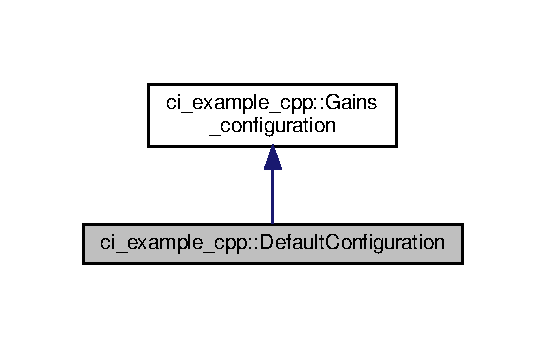
\includegraphics[width=262pt]{classci__example__cpp_1_1DefaultConfiguration__inherit__graph}
\end{center}
\end{figure}


Collaboration diagram for ci\+\_\+example\+\_\+cpp\+:\+:Default\+Configuration\+:
\nopagebreak
\begin{figure}[H]
\begin{center}
\leavevmode
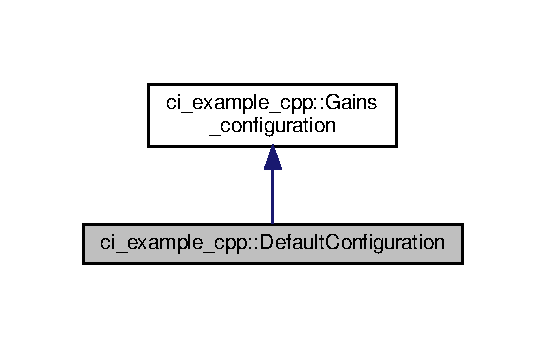
\includegraphics[width=262pt]{classci__example__cpp_1_1DefaultConfiguration__coll__graph}
\end{center}
\end{figure}
\subsection*{Public Member Functions}
\begin{DoxyCompactItemize}
\item 
\hyperlink{classci__example__cpp_1_1DefaultConfiguration_a27c16bc673fbd02ef7cd0b66aa677ec7}{$\sim$\+Default\+Configuration} ()
\begin{DoxyCompactList}\small\item\em Here we use the default destructor. \end{DoxyCompactList}\item 
double \hyperlink{classci__example__cpp_1_1DefaultConfiguration_aed613eb3bec06c4459fa3b9e25aefa7c}{get\+\_\+kp} () const
\begin{DoxyCompactList}\small\item\em Always returns D\+E\+F\+A\+U\+L\+T\+\_\+\+KP. \end{DoxyCompactList}\item 
double \hyperlink{classci__example__cpp_1_1DefaultConfiguration_a5eee0c350de525150b04c81a72cd5932}{get\+\_\+kd} () const
\begin{DoxyCompactList}\small\item\em Always returns D\+E\+F\+A\+U\+L\+T\+\_\+\+KD. \end{DoxyCompactList}\item 
double \hyperlink{classci__example__cpp_1_1DefaultConfiguration_a8853e68911e4fd8baf547ac5cffe38db}{get\+\_\+ki} () const
\begin{DoxyCompactList}\small\item\em Always returns D\+E\+F\+A\+U\+L\+T\+\_\+\+KI. \end{DoxyCompactList}\item 
bool \hyperlink{classci__example__cpp_1_1DefaultConfiguration_aba675295652a7530bbb2148bec700ab0}{has\+\_\+error} () const
\begin{DoxyCompactList}\small\item\em Always returns false. \end{DoxyCompactList}\item 
std\+::string \hyperlink{classci__example__cpp_1_1DefaultConfiguration_a06034c96faa086c539a14643534d5aac}{get\+\_\+error} () const
\begin{DoxyCompactList}\small\item\em Always returns \char`\"{}no error\char`\"{}. \end{DoxyCompactList}\end{DoxyCompactItemize}


\subsection{Detailed Description}
Default configuration for the kp, kd, ki paramters. 

This class initialize the \hyperlink{classci__example__cpp_1_1PID}{P\+ID} gains as follow\+:
\begin{DoxyItemize}
\item kp = D\+E\+F\+A\+U\+L\+T\+\_\+\+KP,
\item kd = D\+E\+F\+A\+U\+L\+T\+\_\+\+KD
\item ki = D\+E\+F\+A\+U\+L\+T\+\_\+\+KI 
\end{DoxyItemize}

\subsection{Constructor \& Destructor Documentation}
\mbox{\Hypertarget{classci__example__cpp_1_1DefaultConfiguration_a27c16bc673fbd02ef7cd0b66aa677ec7}\label{classci__example__cpp_1_1DefaultConfiguration_a27c16bc673fbd02ef7cd0b66aa677ec7}} 
\index{ci\+\_\+example\+\_\+cpp\+::\+Default\+Configuration@{ci\+\_\+example\+\_\+cpp\+::\+Default\+Configuration}!````~Default\+Configuration@{$\sim$\+Default\+Configuration}}
\index{````~Default\+Configuration@{$\sim$\+Default\+Configuration}!ci\+\_\+example\+\_\+cpp\+::\+Default\+Configuration@{ci\+\_\+example\+\_\+cpp\+::\+Default\+Configuration}}
\subsubsection{\texorpdfstring{$\sim$\+Default\+Configuration()}{~DefaultConfiguration()}}
{\footnotesize\ttfamily ci\+\_\+example\+\_\+cpp\+::\+Default\+Configuration\+::$\sim$\+Default\+Configuration (\begin{DoxyParamCaption}{ }\end{DoxyParamCaption})\hspace{0.3cm}{\ttfamily [inline]}}



Here we use the default destructor. 



\subsection{Member Function Documentation}
\mbox{\Hypertarget{classci__example__cpp_1_1DefaultConfiguration_a06034c96faa086c539a14643534d5aac}\label{classci__example__cpp_1_1DefaultConfiguration_a06034c96faa086c539a14643534d5aac}} 
\index{ci\+\_\+example\+\_\+cpp\+::\+Default\+Configuration@{ci\+\_\+example\+\_\+cpp\+::\+Default\+Configuration}!get\+\_\+error@{get\+\_\+error}}
\index{get\+\_\+error@{get\+\_\+error}!ci\+\_\+example\+\_\+cpp\+::\+Default\+Configuration@{ci\+\_\+example\+\_\+cpp\+::\+Default\+Configuration}}
\subsubsection{\texorpdfstring{get\+\_\+error()}{get\_error()}}
{\footnotesize\ttfamily std\+::string ci\+\_\+example\+\_\+cpp\+::\+Default\+Configuration\+::get\+\_\+error (\begin{DoxyParamCaption}{ }\end{DoxyParamCaption}) const\hspace{0.3cm}{\ttfamily [virtual]}}



Always returns \char`\"{}no error\char`\"{}. 

\begin{DoxyReturn}{Returns}
std\+::string \char`\"{}no error\char`\"{} 
\end{DoxyReturn}


Implements \hyperlink{classci__example__cpp_1_1Gains__configuration_a886100ef46082d1b9f8ee169318dc554}{ci\+\_\+example\+\_\+cpp\+::\+Gains\+\_\+configuration}.

\mbox{\Hypertarget{classci__example__cpp_1_1DefaultConfiguration_a5eee0c350de525150b04c81a72cd5932}\label{classci__example__cpp_1_1DefaultConfiguration_a5eee0c350de525150b04c81a72cd5932}} 
\index{ci\+\_\+example\+\_\+cpp\+::\+Default\+Configuration@{ci\+\_\+example\+\_\+cpp\+::\+Default\+Configuration}!get\+\_\+kd@{get\+\_\+kd}}
\index{get\+\_\+kd@{get\+\_\+kd}!ci\+\_\+example\+\_\+cpp\+::\+Default\+Configuration@{ci\+\_\+example\+\_\+cpp\+::\+Default\+Configuration}}
\subsubsection{\texorpdfstring{get\+\_\+kd()}{get\_kd()}}
{\footnotesize\ttfamily double ci\+\_\+example\+\_\+cpp\+::\+Default\+Configuration\+::get\+\_\+kd (\begin{DoxyParamCaption}{ }\end{DoxyParamCaption}) const\hspace{0.3cm}{\ttfamily [virtual]}}



Always returns D\+E\+F\+A\+U\+L\+T\+\_\+\+KD. 

\begin{DoxyReturn}{Returns}
double D\+E\+F\+A\+U\+L\+T\+\_\+\+KD 
\end{DoxyReturn}


Implements \hyperlink{classci__example__cpp_1_1Gains__configuration_a4bc25c0a8283f36366b888feaf15efa9}{ci\+\_\+example\+\_\+cpp\+::\+Gains\+\_\+configuration}.

\mbox{\Hypertarget{classci__example__cpp_1_1DefaultConfiguration_a8853e68911e4fd8baf547ac5cffe38db}\label{classci__example__cpp_1_1DefaultConfiguration_a8853e68911e4fd8baf547ac5cffe38db}} 
\index{ci\+\_\+example\+\_\+cpp\+::\+Default\+Configuration@{ci\+\_\+example\+\_\+cpp\+::\+Default\+Configuration}!get\+\_\+ki@{get\+\_\+ki}}
\index{get\+\_\+ki@{get\+\_\+ki}!ci\+\_\+example\+\_\+cpp\+::\+Default\+Configuration@{ci\+\_\+example\+\_\+cpp\+::\+Default\+Configuration}}
\subsubsection{\texorpdfstring{get\+\_\+ki()}{get\_ki()}}
{\footnotesize\ttfamily double ci\+\_\+example\+\_\+cpp\+::\+Default\+Configuration\+::get\+\_\+ki (\begin{DoxyParamCaption}{ }\end{DoxyParamCaption}) const\hspace{0.3cm}{\ttfamily [virtual]}}



Always returns D\+E\+F\+A\+U\+L\+T\+\_\+\+KI. 

\begin{DoxyReturn}{Returns}
double D\+E\+F\+A\+U\+L\+T\+\_\+\+KI 
\end{DoxyReturn}


Implements \hyperlink{classci__example__cpp_1_1Gains__configuration_a1ac03c97e04ebfbb3c29122e13b0ec0e}{ci\+\_\+example\+\_\+cpp\+::\+Gains\+\_\+configuration}.

\mbox{\Hypertarget{classci__example__cpp_1_1DefaultConfiguration_aed613eb3bec06c4459fa3b9e25aefa7c}\label{classci__example__cpp_1_1DefaultConfiguration_aed613eb3bec06c4459fa3b9e25aefa7c}} 
\index{ci\+\_\+example\+\_\+cpp\+::\+Default\+Configuration@{ci\+\_\+example\+\_\+cpp\+::\+Default\+Configuration}!get\+\_\+kp@{get\+\_\+kp}}
\index{get\+\_\+kp@{get\+\_\+kp}!ci\+\_\+example\+\_\+cpp\+::\+Default\+Configuration@{ci\+\_\+example\+\_\+cpp\+::\+Default\+Configuration}}
\subsubsection{\texorpdfstring{get\+\_\+kp()}{get\_kp()}}
{\footnotesize\ttfamily double ci\+\_\+example\+\_\+cpp\+::\+Default\+Configuration\+::get\+\_\+kp (\begin{DoxyParamCaption}{ }\end{DoxyParamCaption}) const\hspace{0.3cm}{\ttfamily [virtual]}}



Always returns D\+E\+F\+A\+U\+L\+T\+\_\+\+KP. 

\begin{DoxyReturn}{Returns}
double D\+E\+F\+A\+U\+L\+T\+\_\+\+KP 
\end{DoxyReturn}


Implements \hyperlink{classci__example__cpp_1_1Gains__configuration_add5ce511c797cd688e12cee09d8ec0b8}{ci\+\_\+example\+\_\+cpp\+::\+Gains\+\_\+configuration}.

\mbox{\Hypertarget{classci__example__cpp_1_1DefaultConfiguration_aba675295652a7530bbb2148bec700ab0}\label{classci__example__cpp_1_1DefaultConfiguration_aba675295652a7530bbb2148bec700ab0}} 
\index{ci\+\_\+example\+\_\+cpp\+::\+Default\+Configuration@{ci\+\_\+example\+\_\+cpp\+::\+Default\+Configuration}!has\+\_\+error@{has\+\_\+error}}
\index{has\+\_\+error@{has\+\_\+error}!ci\+\_\+example\+\_\+cpp\+::\+Default\+Configuration@{ci\+\_\+example\+\_\+cpp\+::\+Default\+Configuration}}
\subsubsection{\texorpdfstring{has\+\_\+error()}{has\_error()}}
{\footnotesize\ttfamily bool ci\+\_\+example\+\_\+cpp\+::\+Default\+Configuration\+::has\+\_\+error (\begin{DoxyParamCaption}{ }\end{DoxyParamCaption}) const\hspace{0.3cm}{\ttfamily [virtual]}}



Always returns false. 

\begin{DoxyReturn}{Returns}
true Never 

false Always 
\end{DoxyReturn}


Implements \hyperlink{classci__example__cpp_1_1Gains__configuration_ae075925f60288519f8a4fcb477453a66}{ci\+\_\+example\+\_\+cpp\+::\+Gains\+\_\+configuration}.



The documentation for this class was generated from the following files\+:\begin{DoxyCompactItemize}
\item 
include/ci\+\_\+example\+\_\+cpp/\hyperlink{default__configuration_8hpp}{default\+\_\+configuration.\+hpp}\item 
src/\hyperlink{default__configuration_8cpp}{default\+\_\+configuration.\+cpp}\end{DoxyCompactItemize}

\hypertarget{classci__example__cpp_1_1File__configuration}{}\section{ci\+\_\+example\+\_\+cpp\+:\+:File\+\_\+configuration Class Reference}
\label{classci__example__cpp_1_1File__configuration}\index{ci\+\_\+example\+\_\+cpp\+::\+File\+\_\+configuration@{ci\+\_\+example\+\_\+cpp\+::\+File\+\_\+configuration}}


Reading configuration from yaml file.  




{\ttfamily \#include $<$file\+\_\+configuration.\+hpp$>$}



Inheritance diagram for ci\+\_\+example\+\_\+cpp\+:\+:File\+\_\+configuration\+:
\nopagebreak
\begin{figure}[H]
\begin{center}
\leavevmode
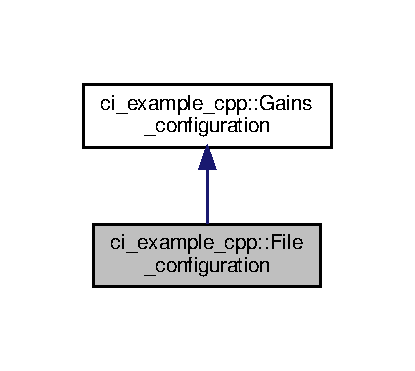
\includegraphics[width=199pt]{classci__example__cpp_1_1File__configuration__inherit__graph}
\end{center}
\end{figure}


Collaboration diagram for ci\+\_\+example\+\_\+cpp\+:\+:File\+\_\+configuration\+:
\nopagebreak
\begin{figure}[H]
\begin{center}
\leavevmode
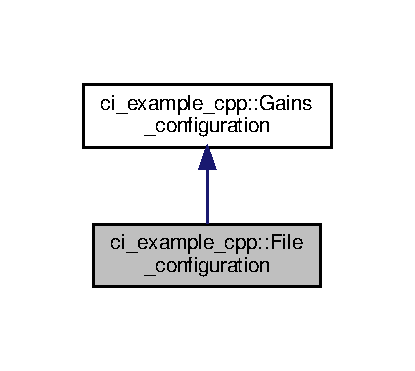
\includegraphics[width=199pt]{classci__example__cpp_1_1File__configuration__coll__graph}
\end{center}
\end{figure}
\subsection*{Public Member Functions}
\begin{DoxyCompactItemize}
\item 
\hyperlink{classci__example__cpp_1_1File__configuration_a9eb17de315392f3f755a327af4beb5d7}{File\+\_\+configuration} (std\+::string yaml\+\_\+file)
\begin{DoxyCompactList}\small\item\em Returns error encountered when reading configuration. \end{DoxyCompactList}\item 
double \hyperlink{classci__example__cpp_1_1File__configuration_a5d051da802569c36feeab2b1fbf9a09a}{get\+\_\+kp} () const
\begin{DoxyCompactList}\small\item\em Get the proportional gain. \end{DoxyCompactList}\item 
double \hyperlink{classci__example__cpp_1_1File__configuration_a14b1e36766d55ee0132a78fbc41f8096}{get\+\_\+kd} () const
\begin{DoxyCompactList}\small\item\em Get the derivative gain. \end{DoxyCompactList}\item 
double \hyperlink{classci__example__cpp_1_1File__configuration_a6e338977105cbcf8b822892d1feb9006}{get\+\_\+ki} () const
\begin{DoxyCompactList}\small\item\em Get the integral gain. \end{DoxyCompactList}\item 
bool \hyperlink{classci__example__cpp_1_1File__configuration_aa3cae137be3b59e61d13c2a9b1ec8b6a}{has\+\_\+error} () const
\begin{DoxyCompactList}\small\item\em Enquire if an error was encountered while reading the configuration. \end{DoxyCompactList}\item 
std\+::string \hyperlink{classci__example__cpp_1_1File__configuration_aaf67f7d61d467563a4dce8aa69306a6a}{get\+\_\+error} () const
\begin{DoxyCompactList}\small\item\em returns error encountered when reading configuration \end{DoxyCompactList}\end{DoxyCompactItemize}
\subsection*{Private Attributes}
\begin{DoxyCompactItemize}
\item 
double \hyperlink{classci__example__cpp_1_1File__configuration_a919075c40e92692f39cb26d99d6c40a9}{kp\+\_\+}
\begin{DoxyCompactList}\small\item\em Proportinal gain. \end{DoxyCompactList}\item 
double \hyperlink{classci__example__cpp_1_1File__configuration_aabec4cb5a29a53e469be722cf2f47fbf}{kd\+\_\+}
\begin{DoxyCompactList}\small\item\em Derivative gain. \end{DoxyCompactList}\item 
double \hyperlink{classci__example__cpp_1_1File__configuration_ae819105d7a538cb7f604824a10f8b814}{ki\+\_\+}
\begin{DoxyCompactList}\small\item\em Integral gain. \end{DoxyCompactList}\item 
std\+::string \hyperlink{classci__example__cpp_1_1File__configuration_aabc2359549686784a62fae2130f1aae7}{error\+\_\+message\+\_\+}
\begin{DoxyCompactList}\small\item\em Internal error message. \end{DoxyCompactList}\item 
bool \hyperlink{classci__example__cpp_1_1File__configuration_a838d95dfb9f01ea950cd67f4c7320eff}{error\+\_\+}
\begin{DoxyCompactList}\small\item\em True if an error occured. \end{DoxyCompactList}\end{DoxyCompactItemize}


\subsection{Detailed Description}
Reading configuration from yaml file. \begin{Desc}
\item[Examples\+: ]\par
\hyperlink{demo_pid_load_from_file_8cpp-example}{demo\+\_\+pid\+\_\+load\+\_\+from\+\_\+file.\+cpp}.\end{Desc}


\subsection{Constructor \& Destructor Documentation}
\mbox{\Hypertarget{classci__example__cpp_1_1File__configuration_a9eb17de315392f3f755a327af4beb5d7}\label{classci__example__cpp_1_1File__configuration_a9eb17de315392f3f755a327af4beb5d7}} 
\index{ci\+\_\+example\+\_\+cpp\+::\+File\+\_\+configuration@{ci\+\_\+example\+\_\+cpp\+::\+File\+\_\+configuration}!File\+\_\+configuration@{File\+\_\+configuration}}
\index{File\+\_\+configuration@{File\+\_\+configuration}!ci\+\_\+example\+\_\+cpp\+::\+File\+\_\+configuration@{ci\+\_\+example\+\_\+cpp\+::\+File\+\_\+configuration}}
\subsubsection{\texorpdfstring{File\+\_\+configuration()}{File\_configuration()}}
{\footnotesize\ttfamily ci\+\_\+example\+\_\+cpp\+::\+File\+\_\+configuration\+::\+File\+\_\+configuration (\begin{DoxyParamCaption}\item[{std\+::string}]{yaml\+\_\+file }\end{DoxyParamCaption})}



Returns error encountered when reading configuration. 


\begin{DoxyParams}{Parameters}
{\em yaml\+\_\+file} & absolute path to configuration yaml file. The file is expected to have parameters \char`\"{}kp\char`\"{}, \char`\"{}kd\char`\"{} and \char`\"{}ki\char`\"{} \\
\hline
\end{DoxyParams}
\begin{DoxySeeAlso}{See also}
\hyperlink{classci__example__cpp_1_1File__configuration_aa3cae137be3b59e61d13c2a9b1ec8b6a}{has\+\_\+error()} 
\end{DoxySeeAlso}


\subsection{Member Function Documentation}
\mbox{\Hypertarget{classci__example__cpp_1_1File__configuration_aaf67f7d61d467563a4dce8aa69306a6a}\label{classci__example__cpp_1_1File__configuration_aaf67f7d61d467563a4dce8aa69306a6a}} 
\index{ci\+\_\+example\+\_\+cpp\+::\+File\+\_\+configuration@{ci\+\_\+example\+\_\+cpp\+::\+File\+\_\+configuration}!get\+\_\+error@{get\+\_\+error}}
\index{get\+\_\+error@{get\+\_\+error}!ci\+\_\+example\+\_\+cpp\+::\+File\+\_\+configuration@{ci\+\_\+example\+\_\+cpp\+::\+File\+\_\+configuration}}
\subsubsection{\texorpdfstring{get\+\_\+error()}{get\_error()}}
{\footnotesize\ttfamily std\+::string ci\+\_\+example\+\_\+cpp\+::\+File\+\_\+configuration\+::get\+\_\+error (\begin{DoxyParamCaption}{ }\end{DoxyParamCaption}) const\hspace{0.3cm}{\ttfamily [virtual]}}



returns error encountered when reading configuration 

\begin{DoxySeeAlso}{See also}
\hyperlink{classci__example__cpp_1_1File__configuration_aa3cae137be3b59e61d13c2a9b1ec8b6a}{has\+\_\+error()} 
\end{DoxySeeAlso}


Implements \hyperlink{classci__example__cpp_1_1Gains__configuration_a886100ef46082d1b9f8ee169318dc554}{ci\+\_\+example\+\_\+cpp\+::\+Gains\+\_\+configuration}.

\begin{Desc}
\item[Examples\+: ]\par
\hyperlink{demo_pid_load_from_file_8cpp-example}{demo\+\_\+pid\+\_\+load\+\_\+from\+\_\+file.\+cpp}.\end{Desc}
\mbox{\Hypertarget{classci__example__cpp_1_1File__configuration_a14b1e36766d55ee0132a78fbc41f8096}\label{classci__example__cpp_1_1File__configuration_a14b1e36766d55ee0132a78fbc41f8096}} 
\index{ci\+\_\+example\+\_\+cpp\+::\+File\+\_\+configuration@{ci\+\_\+example\+\_\+cpp\+::\+File\+\_\+configuration}!get\+\_\+kd@{get\+\_\+kd}}
\index{get\+\_\+kd@{get\+\_\+kd}!ci\+\_\+example\+\_\+cpp\+::\+File\+\_\+configuration@{ci\+\_\+example\+\_\+cpp\+::\+File\+\_\+configuration}}
\subsubsection{\texorpdfstring{get\+\_\+kd()}{get\_kd()}}
{\footnotesize\ttfamily double ci\+\_\+example\+\_\+cpp\+::\+File\+\_\+configuration\+::get\+\_\+kd (\begin{DoxyParamCaption}{ }\end{DoxyParamCaption}) const\hspace{0.3cm}{\ttfamily [virtual]}}



Get the derivative gain. 

\begin{DoxyReturn}{Returns}
double 
\end{DoxyReturn}


Implements \hyperlink{classci__example__cpp_1_1Gains__configuration_a4bc25c0a8283f36366b888feaf15efa9}{ci\+\_\+example\+\_\+cpp\+::\+Gains\+\_\+configuration}.

\mbox{\Hypertarget{classci__example__cpp_1_1File__configuration_a6e338977105cbcf8b822892d1feb9006}\label{classci__example__cpp_1_1File__configuration_a6e338977105cbcf8b822892d1feb9006}} 
\index{ci\+\_\+example\+\_\+cpp\+::\+File\+\_\+configuration@{ci\+\_\+example\+\_\+cpp\+::\+File\+\_\+configuration}!get\+\_\+ki@{get\+\_\+ki}}
\index{get\+\_\+ki@{get\+\_\+ki}!ci\+\_\+example\+\_\+cpp\+::\+File\+\_\+configuration@{ci\+\_\+example\+\_\+cpp\+::\+File\+\_\+configuration}}
\subsubsection{\texorpdfstring{get\+\_\+ki()}{get\_ki()}}
{\footnotesize\ttfamily double ci\+\_\+example\+\_\+cpp\+::\+File\+\_\+configuration\+::get\+\_\+ki (\begin{DoxyParamCaption}{ }\end{DoxyParamCaption}) const\hspace{0.3cm}{\ttfamily [virtual]}}



Get the integral gain. 

\begin{DoxyReturn}{Returns}
double 
\end{DoxyReturn}


Implements \hyperlink{classci__example__cpp_1_1Gains__configuration_a1ac03c97e04ebfbb3c29122e13b0ec0e}{ci\+\_\+example\+\_\+cpp\+::\+Gains\+\_\+configuration}.

\mbox{\Hypertarget{classci__example__cpp_1_1File__configuration_a5d051da802569c36feeab2b1fbf9a09a}\label{classci__example__cpp_1_1File__configuration_a5d051da802569c36feeab2b1fbf9a09a}} 
\index{ci\+\_\+example\+\_\+cpp\+::\+File\+\_\+configuration@{ci\+\_\+example\+\_\+cpp\+::\+File\+\_\+configuration}!get\+\_\+kp@{get\+\_\+kp}}
\index{get\+\_\+kp@{get\+\_\+kp}!ci\+\_\+example\+\_\+cpp\+::\+File\+\_\+configuration@{ci\+\_\+example\+\_\+cpp\+::\+File\+\_\+configuration}}
\subsubsection{\texorpdfstring{get\+\_\+kp()}{get\_kp()}}
{\footnotesize\ttfamily double ci\+\_\+example\+\_\+cpp\+::\+File\+\_\+configuration\+::get\+\_\+kp (\begin{DoxyParamCaption}{ }\end{DoxyParamCaption}) const\hspace{0.3cm}{\ttfamily [virtual]}}



Get the proportional gain. 

\begin{DoxyReturn}{Returns}
double 
\end{DoxyReturn}


Implements \hyperlink{classci__example__cpp_1_1Gains__configuration_add5ce511c797cd688e12cee09d8ec0b8}{ci\+\_\+example\+\_\+cpp\+::\+Gains\+\_\+configuration}.

\mbox{\Hypertarget{classci__example__cpp_1_1File__configuration_aa3cae137be3b59e61d13c2a9b1ec8b6a}\label{classci__example__cpp_1_1File__configuration_aa3cae137be3b59e61d13c2a9b1ec8b6a}} 
\index{ci\+\_\+example\+\_\+cpp\+::\+File\+\_\+configuration@{ci\+\_\+example\+\_\+cpp\+::\+File\+\_\+configuration}!has\+\_\+error@{has\+\_\+error}}
\index{has\+\_\+error@{has\+\_\+error}!ci\+\_\+example\+\_\+cpp\+::\+File\+\_\+configuration@{ci\+\_\+example\+\_\+cpp\+::\+File\+\_\+configuration}}
\subsubsection{\texorpdfstring{has\+\_\+error()}{has\_error()}}
{\footnotesize\ttfamily bool ci\+\_\+example\+\_\+cpp\+::\+File\+\_\+configuration\+::has\+\_\+error (\begin{DoxyParamCaption}{ }\end{DoxyParamCaption}) const\hspace{0.3cm}{\ttfamily [virtual]}}



Enquire if an error was encountered while reading the configuration. 

\begin{DoxySeeAlso}{See also}
\hyperlink{classci__example__cpp_1_1File__configuration_aaf67f7d61d467563a4dce8aa69306a6a}{get\+\_\+error()} 
\end{DoxySeeAlso}
\begin{DoxyReturn}{Returns}
true if an error has been encountered 

false otherwise 
\end{DoxyReturn}


Implements \hyperlink{classci__example__cpp_1_1Gains__configuration_ae075925f60288519f8a4fcb477453a66}{ci\+\_\+example\+\_\+cpp\+::\+Gains\+\_\+configuration}.

\begin{Desc}
\item[Examples\+: ]\par
\hyperlink{demo_pid_load_from_file_8cpp-example}{demo\+\_\+pid\+\_\+load\+\_\+from\+\_\+file.\+cpp}.\end{Desc}


\subsection{Member Data Documentation}
\mbox{\Hypertarget{classci__example__cpp_1_1File__configuration_a838d95dfb9f01ea950cd67f4c7320eff}\label{classci__example__cpp_1_1File__configuration_a838d95dfb9f01ea950cd67f4c7320eff}} 
\index{ci\+\_\+example\+\_\+cpp\+::\+File\+\_\+configuration@{ci\+\_\+example\+\_\+cpp\+::\+File\+\_\+configuration}!error\+\_\+@{error\+\_\+}}
\index{error\+\_\+@{error\+\_\+}!ci\+\_\+example\+\_\+cpp\+::\+File\+\_\+configuration@{ci\+\_\+example\+\_\+cpp\+::\+File\+\_\+configuration}}
\subsubsection{\texorpdfstring{error\+\_\+}{error\_}}
{\footnotesize\ttfamily bool ci\+\_\+example\+\_\+cpp\+::\+File\+\_\+configuration\+::error\+\_\+\hspace{0.3cm}{\ttfamily [private]}}



True if an error occured. 

\mbox{\Hypertarget{classci__example__cpp_1_1File__configuration_aabc2359549686784a62fae2130f1aae7}\label{classci__example__cpp_1_1File__configuration_aabc2359549686784a62fae2130f1aae7}} 
\index{ci\+\_\+example\+\_\+cpp\+::\+File\+\_\+configuration@{ci\+\_\+example\+\_\+cpp\+::\+File\+\_\+configuration}!error\+\_\+message\+\_\+@{error\+\_\+message\+\_\+}}
\index{error\+\_\+message\+\_\+@{error\+\_\+message\+\_\+}!ci\+\_\+example\+\_\+cpp\+::\+File\+\_\+configuration@{ci\+\_\+example\+\_\+cpp\+::\+File\+\_\+configuration}}
\subsubsection{\texorpdfstring{error\+\_\+message\+\_\+}{error\_message\_}}
{\footnotesize\ttfamily std\+::string ci\+\_\+example\+\_\+cpp\+::\+File\+\_\+configuration\+::error\+\_\+message\+\_\+\hspace{0.3cm}{\ttfamily [private]}}



Internal error message. 

\mbox{\Hypertarget{classci__example__cpp_1_1File__configuration_aabec4cb5a29a53e469be722cf2f47fbf}\label{classci__example__cpp_1_1File__configuration_aabec4cb5a29a53e469be722cf2f47fbf}} 
\index{ci\+\_\+example\+\_\+cpp\+::\+File\+\_\+configuration@{ci\+\_\+example\+\_\+cpp\+::\+File\+\_\+configuration}!kd\+\_\+@{kd\+\_\+}}
\index{kd\+\_\+@{kd\+\_\+}!ci\+\_\+example\+\_\+cpp\+::\+File\+\_\+configuration@{ci\+\_\+example\+\_\+cpp\+::\+File\+\_\+configuration}}
\subsubsection{\texorpdfstring{kd\+\_\+}{kd\_}}
{\footnotesize\ttfamily double ci\+\_\+example\+\_\+cpp\+::\+File\+\_\+configuration\+::kd\+\_\+\hspace{0.3cm}{\ttfamily [private]}}



Derivative gain. 

\mbox{\Hypertarget{classci__example__cpp_1_1File__configuration_ae819105d7a538cb7f604824a10f8b814}\label{classci__example__cpp_1_1File__configuration_ae819105d7a538cb7f604824a10f8b814}} 
\index{ci\+\_\+example\+\_\+cpp\+::\+File\+\_\+configuration@{ci\+\_\+example\+\_\+cpp\+::\+File\+\_\+configuration}!ki\+\_\+@{ki\+\_\+}}
\index{ki\+\_\+@{ki\+\_\+}!ci\+\_\+example\+\_\+cpp\+::\+File\+\_\+configuration@{ci\+\_\+example\+\_\+cpp\+::\+File\+\_\+configuration}}
\subsubsection{\texorpdfstring{ki\+\_\+}{ki\_}}
{\footnotesize\ttfamily double ci\+\_\+example\+\_\+cpp\+::\+File\+\_\+configuration\+::ki\+\_\+\hspace{0.3cm}{\ttfamily [private]}}



Integral gain. 

\mbox{\Hypertarget{classci__example__cpp_1_1File__configuration_a919075c40e92692f39cb26d99d6c40a9}\label{classci__example__cpp_1_1File__configuration_a919075c40e92692f39cb26d99d6c40a9}} 
\index{ci\+\_\+example\+\_\+cpp\+::\+File\+\_\+configuration@{ci\+\_\+example\+\_\+cpp\+::\+File\+\_\+configuration}!kp\+\_\+@{kp\+\_\+}}
\index{kp\+\_\+@{kp\+\_\+}!ci\+\_\+example\+\_\+cpp\+::\+File\+\_\+configuration@{ci\+\_\+example\+\_\+cpp\+::\+File\+\_\+configuration}}
\subsubsection{\texorpdfstring{kp\+\_\+}{kp\_}}
{\footnotesize\ttfamily double ci\+\_\+example\+\_\+cpp\+::\+File\+\_\+configuration\+::kp\+\_\+\hspace{0.3cm}{\ttfamily [private]}}



Proportinal gain. 



The documentation for this class was generated from the following files\+:\begin{DoxyCompactItemize}
\item 
include/ci\+\_\+example\+\_\+cpp/\hyperlink{file__configuration_8hpp}{file\+\_\+configuration.\+hpp}\item 
src/\hyperlink{file__configuration_8cpp}{file\+\_\+configuration.\+cpp}\end{DoxyCompactItemize}

\hypertarget{classci__example__cpp_1_1Gains__configuration}{}\section{ci\+\_\+example\+\_\+cpp\+:\+:Gains\+\_\+configuration Class Reference}
\label{classci__example__cpp_1_1Gains__configuration}\index{ci\+\_\+example\+\_\+cpp\+::\+Gains\+\_\+configuration@{ci\+\_\+example\+\_\+cpp\+::\+Gains\+\_\+configuration}}


Abstract class defining for the \hyperlink{classci__example__cpp_1_1PID}{P\+ID} configuration.  




{\ttfamily \#include $<$gains\+\_\+configuration.\+hpp$>$}



Inheritance diagram for ci\+\_\+example\+\_\+cpp\+:\+:Gains\+\_\+configuration\+:
\nopagebreak
\begin{figure}[H]
\begin{center}
\leavevmode
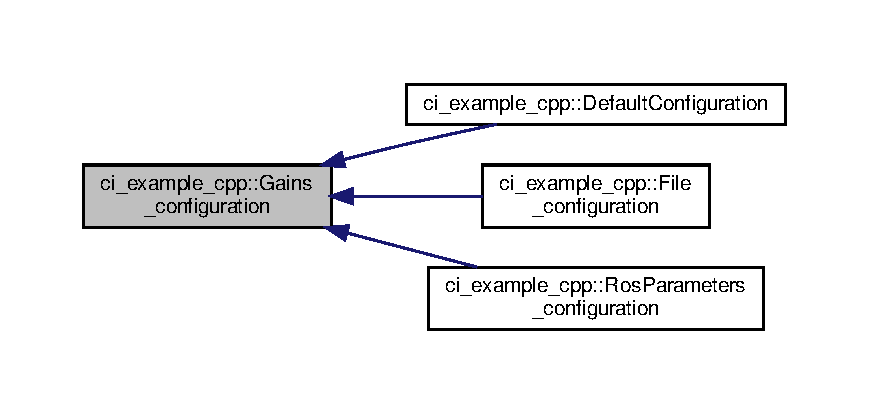
\includegraphics[width=350pt]{classci__example__cpp_1_1Gains__configuration__inherit__graph}
\end{center}
\end{figure}
\subsection*{Public Member Functions}
\begin{DoxyCompactItemize}
\item 
\mbox{\Hypertarget{classci__example__cpp_1_1Gains__configuration_a14a531c18d485164e218112a1f3bbc39}\label{classci__example__cpp_1_1Gains__configuration_a14a531c18d485164e218112a1f3bbc39}} 
virtual \hyperlink{classci__example__cpp_1_1Gains__configuration_a14a531c18d485164e218112a1f3bbc39}{$\sim$\+Gains\+\_\+configuration} ()
\begin{DoxyCompactList}\small\item\em The default destructor do nothing. \end{DoxyCompactList}\item 
virtual double \hyperlink{classci__example__cpp_1_1Gains__configuration_add5ce511c797cd688e12cee09d8ec0b8}{get\+\_\+kp} () const =0
\begin{DoxyCompactList}\small\item\em Get the proportional gain. \end{DoxyCompactList}\item 
virtual double \hyperlink{classci__example__cpp_1_1Gains__configuration_a4bc25c0a8283f36366b888feaf15efa9}{get\+\_\+kd} () const =0
\begin{DoxyCompactList}\small\item\em Get the derivative gain. \end{DoxyCompactList}\item 
virtual double \hyperlink{classci__example__cpp_1_1Gains__configuration_a1ac03c97e04ebfbb3c29122e13b0ec0e}{get\+\_\+ki} () const =0
\begin{DoxyCompactList}\small\item\em Get the integral gain. \end{DoxyCompactList}\item 
virtual bool \hyperlink{classci__example__cpp_1_1Gains__configuration_ae075925f60288519f8a4fcb477453a66}{has\+\_\+error} () const =0
\begin{DoxyCompactList}\small\item\em Enquire if an error was encountered while reading the configuration. \end{DoxyCompactList}\item 
virtual std\+::string \hyperlink{classci__example__cpp_1_1Gains__configuration_a886100ef46082d1b9f8ee169318dc554}{get\+\_\+error} () const =0
\begin{DoxyCompactList}\small\item\em returns error encountered when reading configuration \end{DoxyCompactList}\end{DoxyCompactItemize}


\subsection{Detailed Description}
Abstract class defining for the \hyperlink{classci__example__cpp_1_1PID}{P\+ID} configuration. 

This virtual object describes the configuration a \hyperlink{classci__example__cpp_1_1PID}{P\+ID} objects is waiting for. Daughter class will for example be initialize through files, R\+OS params, etc. 

\subsection{Member Function Documentation}
\mbox{\Hypertarget{classci__example__cpp_1_1Gains__configuration_a886100ef46082d1b9f8ee169318dc554}\label{classci__example__cpp_1_1Gains__configuration_a886100ef46082d1b9f8ee169318dc554}} 
\index{ci\+\_\+example\+\_\+cpp\+::\+Gains\+\_\+configuration@{ci\+\_\+example\+\_\+cpp\+::\+Gains\+\_\+configuration}!get\+\_\+error@{get\+\_\+error}}
\index{get\+\_\+error@{get\+\_\+error}!ci\+\_\+example\+\_\+cpp\+::\+Gains\+\_\+configuration@{ci\+\_\+example\+\_\+cpp\+::\+Gains\+\_\+configuration}}
\subsubsection{\texorpdfstring{get\+\_\+error()}{get\_error()}}
{\footnotesize\ttfamily virtual std\+::string ci\+\_\+example\+\_\+cpp\+::\+Gains\+\_\+configuration\+::get\+\_\+error (\begin{DoxyParamCaption}{ }\end{DoxyParamCaption}) const\hspace{0.3cm}{\ttfamily [pure virtual]}}



returns error encountered when reading configuration 

\begin{DoxySeeAlso}{See also}
\hyperlink{classci__example__cpp_1_1Gains__configuration_ae075925f60288519f8a4fcb477453a66}{has\+\_\+error()} 
\end{DoxySeeAlso}


Implemented in \hyperlink{classci__example__cpp_1_1DefaultConfiguration_a06034c96faa086c539a14643534d5aac}{ci\+\_\+example\+\_\+cpp\+::\+Default\+Configuration}, \hyperlink{classci__example__cpp_1_1RosParameters__configuration_aa6c44530007d18df221b22b84abcedea}{ci\+\_\+example\+\_\+cpp\+::\+Ros\+Parameters\+\_\+configuration}, and \hyperlink{classci__example__cpp_1_1File__configuration_aaf67f7d61d467563a4dce8aa69306a6a}{ci\+\_\+example\+\_\+cpp\+::\+File\+\_\+configuration}.

\mbox{\Hypertarget{classci__example__cpp_1_1Gains__configuration_a4bc25c0a8283f36366b888feaf15efa9}\label{classci__example__cpp_1_1Gains__configuration_a4bc25c0a8283f36366b888feaf15efa9}} 
\index{ci\+\_\+example\+\_\+cpp\+::\+Gains\+\_\+configuration@{ci\+\_\+example\+\_\+cpp\+::\+Gains\+\_\+configuration}!get\+\_\+kd@{get\+\_\+kd}}
\index{get\+\_\+kd@{get\+\_\+kd}!ci\+\_\+example\+\_\+cpp\+::\+Gains\+\_\+configuration@{ci\+\_\+example\+\_\+cpp\+::\+Gains\+\_\+configuration}}
\subsubsection{\texorpdfstring{get\+\_\+kd()}{get\_kd()}}
{\footnotesize\ttfamily virtual double ci\+\_\+example\+\_\+cpp\+::\+Gains\+\_\+configuration\+::get\+\_\+kd (\begin{DoxyParamCaption}{ }\end{DoxyParamCaption}) const\hspace{0.3cm}{\ttfamily [pure virtual]}}



Get the derivative gain. 

\begin{DoxyReturn}{Returns}
double 
\end{DoxyReturn}


Implemented in \hyperlink{classci__example__cpp_1_1DefaultConfiguration_a5eee0c350de525150b04c81a72cd5932}{ci\+\_\+example\+\_\+cpp\+::\+Default\+Configuration}, \hyperlink{classci__example__cpp_1_1RosParameters__configuration_a90eb8bc0d9b4b663cde21fe07d44847e}{ci\+\_\+example\+\_\+cpp\+::\+Ros\+Parameters\+\_\+configuration}, and \hyperlink{classci__example__cpp_1_1File__configuration_a14b1e36766d55ee0132a78fbc41f8096}{ci\+\_\+example\+\_\+cpp\+::\+File\+\_\+configuration}.

\mbox{\Hypertarget{classci__example__cpp_1_1Gains__configuration_a1ac03c97e04ebfbb3c29122e13b0ec0e}\label{classci__example__cpp_1_1Gains__configuration_a1ac03c97e04ebfbb3c29122e13b0ec0e}} 
\index{ci\+\_\+example\+\_\+cpp\+::\+Gains\+\_\+configuration@{ci\+\_\+example\+\_\+cpp\+::\+Gains\+\_\+configuration}!get\+\_\+ki@{get\+\_\+ki}}
\index{get\+\_\+ki@{get\+\_\+ki}!ci\+\_\+example\+\_\+cpp\+::\+Gains\+\_\+configuration@{ci\+\_\+example\+\_\+cpp\+::\+Gains\+\_\+configuration}}
\subsubsection{\texorpdfstring{get\+\_\+ki()}{get\_ki()}}
{\footnotesize\ttfamily virtual double ci\+\_\+example\+\_\+cpp\+::\+Gains\+\_\+configuration\+::get\+\_\+ki (\begin{DoxyParamCaption}{ }\end{DoxyParamCaption}) const\hspace{0.3cm}{\ttfamily [pure virtual]}}



Get the integral gain. 

\begin{DoxyReturn}{Returns}
double 
\end{DoxyReturn}


Implemented in \hyperlink{classci__example__cpp_1_1DefaultConfiguration_a8853e68911e4fd8baf547ac5cffe38db}{ci\+\_\+example\+\_\+cpp\+::\+Default\+Configuration}, \hyperlink{classci__example__cpp_1_1RosParameters__configuration_a01be945f19c9fc4734f28460a335e731}{ci\+\_\+example\+\_\+cpp\+::\+Ros\+Parameters\+\_\+configuration}, and \hyperlink{classci__example__cpp_1_1File__configuration_a6e338977105cbcf8b822892d1feb9006}{ci\+\_\+example\+\_\+cpp\+::\+File\+\_\+configuration}.

\mbox{\Hypertarget{classci__example__cpp_1_1Gains__configuration_add5ce511c797cd688e12cee09d8ec0b8}\label{classci__example__cpp_1_1Gains__configuration_add5ce511c797cd688e12cee09d8ec0b8}} 
\index{ci\+\_\+example\+\_\+cpp\+::\+Gains\+\_\+configuration@{ci\+\_\+example\+\_\+cpp\+::\+Gains\+\_\+configuration}!get\+\_\+kp@{get\+\_\+kp}}
\index{get\+\_\+kp@{get\+\_\+kp}!ci\+\_\+example\+\_\+cpp\+::\+Gains\+\_\+configuration@{ci\+\_\+example\+\_\+cpp\+::\+Gains\+\_\+configuration}}
\subsubsection{\texorpdfstring{get\+\_\+kp()}{get\_kp()}}
{\footnotesize\ttfamily virtual double ci\+\_\+example\+\_\+cpp\+::\+Gains\+\_\+configuration\+::get\+\_\+kp (\begin{DoxyParamCaption}{ }\end{DoxyParamCaption}) const\hspace{0.3cm}{\ttfamily [pure virtual]}}



Get the proportional gain. 

\begin{DoxyReturn}{Returns}
double 
\end{DoxyReturn}


Implemented in \hyperlink{classci__example__cpp_1_1DefaultConfiguration_aed613eb3bec06c4459fa3b9e25aefa7c}{ci\+\_\+example\+\_\+cpp\+::\+Default\+Configuration}, \hyperlink{classci__example__cpp_1_1RosParameters__configuration_a49ccc6c0db59063f1475f08dce23ee5d}{ci\+\_\+example\+\_\+cpp\+::\+Ros\+Parameters\+\_\+configuration}, and \hyperlink{classci__example__cpp_1_1File__configuration_a5d051da802569c36feeab2b1fbf9a09a}{ci\+\_\+example\+\_\+cpp\+::\+File\+\_\+configuration}.

\mbox{\Hypertarget{classci__example__cpp_1_1Gains__configuration_ae075925f60288519f8a4fcb477453a66}\label{classci__example__cpp_1_1Gains__configuration_ae075925f60288519f8a4fcb477453a66}} 
\index{ci\+\_\+example\+\_\+cpp\+::\+Gains\+\_\+configuration@{ci\+\_\+example\+\_\+cpp\+::\+Gains\+\_\+configuration}!has\+\_\+error@{has\+\_\+error}}
\index{has\+\_\+error@{has\+\_\+error}!ci\+\_\+example\+\_\+cpp\+::\+Gains\+\_\+configuration@{ci\+\_\+example\+\_\+cpp\+::\+Gains\+\_\+configuration}}
\subsubsection{\texorpdfstring{has\+\_\+error()}{has\_error()}}
{\footnotesize\ttfamily virtual bool ci\+\_\+example\+\_\+cpp\+::\+Gains\+\_\+configuration\+::has\+\_\+error (\begin{DoxyParamCaption}{ }\end{DoxyParamCaption}) const\hspace{0.3cm}{\ttfamily [pure virtual]}}



Enquire if an error was encountered while reading the configuration. 

\begin{DoxySeeAlso}{See also}
\hyperlink{classci__example__cpp_1_1Gains__configuration_a886100ef46082d1b9f8ee169318dc554}{get\+\_\+error()} 
\end{DoxySeeAlso}
\begin{DoxyReturn}{Returns}
true if an error has been encountered 

false otherwise 
\end{DoxyReturn}


Implemented in \hyperlink{classci__example__cpp_1_1DefaultConfiguration_aba675295652a7530bbb2148bec700ab0}{ci\+\_\+example\+\_\+cpp\+::\+Default\+Configuration}, \hyperlink{classci__example__cpp_1_1RosParameters__configuration_afcf30b3c93eb3d215d8dfb852eaaae52}{ci\+\_\+example\+\_\+cpp\+::\+Ros\+Parameters\+\_\+configuration}, and \hyperlink{classci__example__cpp_1_1File__configuration_aa3cae137be3b59e61d13c2a9b1ec8b6a}{ci\+\_\+example\+\_\+cpp\+::\+File\+\_\+configuration}.



The documentation for this class was generated from the following file\+:\begin{DoxyCompactItemize}
\item 
include/ci\+\_\+example\+\_\+cpp/\hyperlink{gains__configuration_8hpp}{gains\+\_\+configuration.\+hpp}\end{DoxyCompactItemize}

\hypertarget{classci__example__cpp_1_1PID}{}\section{ci\+\_\+example\+\_\+cpp\+:\+:P\+ID Class Reference}
\label{classci__example__cpp_1_1PID}\index{ci\+\_\+example\+\_\+cpp\+::\+P\+ID@{ci\+\_\+example\+\_\+cpp\+::\+P\+ID}}


Simple 1D pid controller.  




{\ttfamily \#include $<$pid.\+hpp$>$}



Collaboration diagram for ci\+\_\+example\+\_\+cpp\+:\+:P\+ID\+:
\nopagebreak
\begin{figure}[H]
\begin{center}
\leavevmode
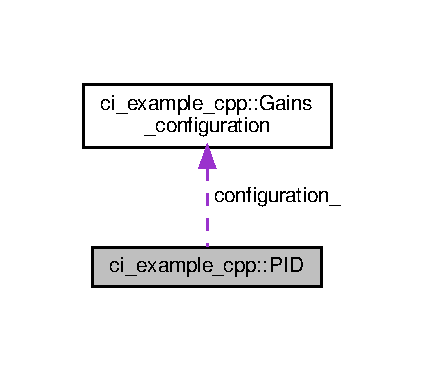
\includegraphics[width=204pt]{classci__example__cpp_1_1PID__coll__graph}
\end{center}
\end{figure}
\subsection*{Public Member Functions}
\begin{DoxyCompactItemize}
\item 
\mbox{\Hypertarget{classci__example__cpp_1_1PID_a8e82fde951fff38658098ff84bbb5cbe}\label{classci__example__cpp_1_1PID_a8e82fde951fff38658098ff84bbb5cbe}} 
\hyperlink{classci__example__cpp_1_1PID_a8e82fde951fff38658098ff84bbb5cbe}{P\+ID} ()
\begin{DoxyCompactList}\small\item\em Construct a default \hyperlink{classci__example__cpp_1_1PID}{P\+ID} object using the \hyperlink{classci__example__cpp_1_1DefaultConfiguration}{Default\+Configuration}. \end{DoxyCompactList}\item 
\hyperlink{classci__example__cpp_1_1PID_a5bbb703065bfd4c49b8d21e02d481c3d}{P\+ID} (const \hyperlink{classci__example__cpp_1_1Gains__configuration}{Gains\+\_\+configuration} \&configuration)
\begin{DoxyCompactList}\small\item\em Construct a new \hyperlink{classci__example__cpp_1_1PID}{P\+ID} object using a user provided configuration. \end{DoxyCompactList}\item 
double \hyperlink{classci__example__cpp_1_1PID_a75a4ccf0455e48e84af23e1d28b0337d}{compute} (const double position, const double velocity, const double position\+\_\+target, const double delta\+\_\+time)
\begin{DoxyCompactList}\small\item\em compute the force related to the pid controller. \end{DoxyCompactList}\item 
void \hyperlink{classci__example__cpp_1_1PID_a65d98fccd38cc385debc3d15670caf0e}{reset\+\_\+integral} ()
\end{DoxyCompactItemize}
\subsection*{Private Attributes}
\begin{DoxyCompactItemize}
\item 
\mbox{\Hypertarget{classci__example__cpp_1_1PID_ad289b145cf9572e57c5c691c065643b7}\label{classci__example__cpp_1_1PID_ad289b145cf9572e57c5c691c065643b7}} 
const \hyperlink{classci__example__cpp_1_1Gains__configuration}{Gains\+\_\+configuration} $\ast$ {\bfseries configuration\+\_\+}
\item 
\mbox{\Hypertarget{classci__example__cpp_1_1PID_a005833b068e3b78b6715599859202ebe}\label{classci__example__cpp_1_1PID_a005833b068e3b78b6715599859202ebe}} 
bool {\bfseries private\+\_\+configuration\+\_\+}
\item 
\mbox{\Hypertarget{classci__example__cpp_1_1PID_aebc028e332ec559269e2623de62c4cea}\label{classci__example__cpp_1_1PID_aebc028e332ec559269e2623de62c4cea}} 
double {\bfseries integral\+\_\+}
\end{DoxyCompactItemize}


\subsection{Detailed Description}
Simple 1D pid controller. \begin{Desc}
\item[Examples\+: ]\par
\hyperlink{demo_pid_8cpp-example}{demo\+\_\+pid.\+cpp}, and \hyperlink{demo_pid_load_from_file_8cpp-example}{demo\+\_\+pid\+\_\+load\+\_\+from\+\_\+file.\+cpp}.\end{Desc}


\subsection{Constructor \& Destructor Documentation}
\mbox{\Hypertarget{classci__example__cpp_1_1PID_a5bbb703065bfd4c49b8d21e02d481c3d}\label{classci__example__cpp_1_1PID_a5bbb703065bfd4c49b8d21e02d481c3d}} 
\index{ci\+\_\+example\+\_\+cpp\+::\+P\+ID@{ci\+\_\+example\+\_\+cpp\+::\+P\+ID}!P\+ID@{P\+ID}}
\index{P\+ID@{P\+ID}!ci\+\_\+example\+\_\+cpp\+::\+P\+ID@{ci\+\_\+example\+\_\+cpp\+::\+P\+ID}}
\subsubsection{\texorpdfstring{P\+I\+D()}{PID()}}
{\footnotesize\ttfamily ci\+\_\+example\+\_\+cpp\+::\+P\+I\+D\+::\+P\+ID (\begin{DoxyParamCaption}\item[{const \hyperlink{classci__example__cpp_1_1Gains__configuration}{Gains\+\_\+configuration} \&}]{configuration }\end{DoxyParamCaption})}



Construct a new \hyperlink{classci__example__cpp_1_1PID}{P\+ID} object using a user provided configuration. 


\begin{DoxyParams}{Parameters}
{\em configuration} & \\
\hline
\end{DoxyParams}


\subsection{Member Function Documentation}
\mbox{\Hypertarget{classci__example__cpp_1_1PID_a75a4ccf0455e48e84af23e1d28b0337d}\label{classci__example__cpp_1_1PID_a75a4ccf0455e48e84af23e1d28b0337d}} 
\index{ci\+\_\+example\+\_\+cpp\+::\+P\+ID@{ci\+\_\+example\+\_\+cpp\+::\+P\+ID}!compute@{compute}}
\index{compute@{compute}!ci\+\_\+example\+\_\+cpp\+::\+P\+ID@{ci\+\_\+example\+\_\+cpp\+::\+P\+ID}}
\subsubsection{\texorpdfstring{compute()}{compute()}}
{\footnotesize\ttfamily double ci\+\_\+example\+\_\+cpp\+::\+P\+I\+D\+::compute (\begin{DoxyParamCaption}\item[{const double}]{position,  }\item[{const double}]{velocity,  }\item[{const double}]{position\+\_\+target,  }\item[{const double}]{delta\+\_\+time }\end{DoxyParamCaption})}



compute the force related to the pid controller. 

\begin{DoxyWarning}{Warning}
this function is not stateless, as it performs integration. Call reset\+\_\+pid() to reset the integral part. 
\end{DoxyWarning}

\begin{DoxyParams}{Parameters}
{\em position} & current position \\
\hline
{\em velocity} & current velocity \\
\hline
{\em position\+\_\+target} & target position \\
\hline
{\em delta\+\_\+time} & time passed since last measurement. Used for integral computation \\
\hline
\end{DoxyParams}
\begin{DoxyReturn}{Returns}
computed force 
\end{DoxyReturn}
\begin{Desc}
\item[Examples\+: ]\par
\hyperlink{demo_pid_8cpp-example}{demo\+\_\+pid.\+cpp}.\end{Desc}
\mbox{\Hypertarget{classci__example__cpp_1_1PID_a65d98fccd38cc385debc3d15670caf0e}\label{classci__example__cpp_1_1PID_a65d98fccd38cc385debc3d15670caf0e}} 
\index{ci\+\_\+example\+\_\+cpp\+::\+P\+ID@{ci\+\_\+example\+\_\+cpp\+::\+P\+ID}!reset\+\_\+integral@{reset\+\_\+integral}}
\index{reset\+\_\+integral@{reset\+\_\+integral}!ci\+\_\+example\+\_\+cpp\+::\+P\+ID@{ci\+\_\+example\+\_\+cpp\+::\+P\+ID}}
\subsubsection{\texorpdfstring{reset\+\_\+integral()}{reset\_integral()}}
{\footnotesize\ttfamily void ci\+\_\+example\+\_\+cpp\+::\+P\+I\+D\+::reset\+\_\+integral (\begin{DoxyParamCaption}{ }\end{DoxyParamCaption})}

reset integral part of the \hyperlink{classci__example__cpp_1_1PID}{P\+ID} \begin{Desc}
\item[Examples\+: ]\par
\hyperlink{demo_pid_8cpp-example}{demo\+\_\+pid.\+cpp}.\end{Desc}


The documentation for this class was generated from the following files\+:\begin{DoxyCompactItemize}
\item 
include/ci\+\_\+example\+\_\+cpp/\hyperlink{pid_8hpp}{pid.\+hpp}\item 
src/\hyperlink{pid_8cpp}{pid.\+cpp}\end{DoxyCompactItemize}

\hypertarget{classci__example__cpp_1_1RosParameters__configuration}{}\section{ci\+\_\+example\+\_\+cpp\+:\+:Ros\+Parameters\+\_\+configuration Class Reference}
\label{classci__example__cpp_1_1RosParameters__configuration}\index{ci\+\_\+example\+\_\+cpp\+::\+Ros\+Parameters\+\_\+configuration@{ci\+\_\+example\+\_\+cpp\+::\+Ros\+Parameters\+\_\+configuration}}


Read gains configuration from the ros parameter server.  




{\ttfamily \#include $<$rosparameters\+\_\+configuration.\+hpp$>$}



Inheritance diagram for ci\+\_\+example\+\_\+cpp\+:\+:Ros\+Parameters\+\_\+configuration\+:
\nopagebreak
\begin{figure}[H]
\begin{center}
\leavevmode
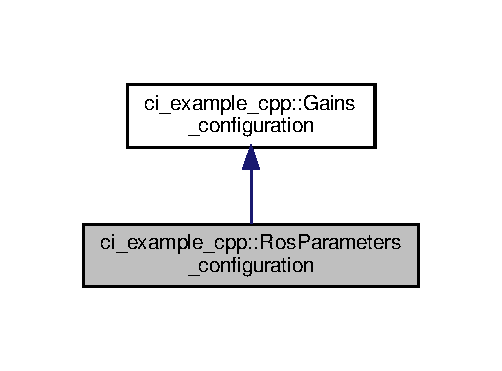
\includegraphics[width=241pt]{classci__example__cpp_1_1RosParameters__configuration__inherit__graph}
\end{center}
\end{figure}


Collaboration diagram for ci\+\_\+example\+\_\+cpp\+:\+:Ros\+Parameters\+\_\+configuration\+:
\nopagebreak
\begin{figure}[H]
\begin{center}
\leavevmode
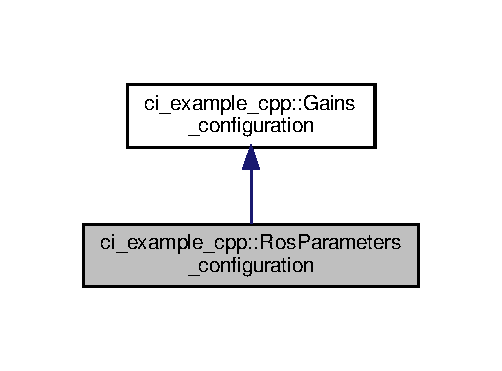
\includegraphics[width=241pt]{classci__example__cpp_1_1RosParameters__configuration__coll__graph}
\end{center}
\end{figure}
\subsection*{Public Member Functions}
\begin{DoxyCompactItemize}
\item 
\hyperlink{classci__example__cpp_1_1RosParameters__configuration_aca978c1389d0f672f9cf2e9a68b131c3}{Ros\+Parameters\+\_\+configuration} ()
\begin{DoxyCompactList}\small\item\em Attempt to get the gains from the parameter server (\char`\"{}gains\+\_\+kp\char`\"{},\char`\"{}gains\+\_\+kd\char`\"{},\char`\"{}gains\+\_\+ki\char`\"{} parameters) If roscore is running, calls to this constructor will be blocking until all the gains are read or roscore is turned off. \end{DoxyCompactList}\item 
\mbox{\Hypertarget{classci__example__cpp_1_1RosParameters__configuration_a49ccc6c0db59063f1475f08dce23ee5d}\label{classci__example__cpp_1_1RosParameters__configuration_a49ccc6c0db59063f1475f08dce23ee5d}} 
double \hyperlink{classci__example__cpp_1_1RosParameters__configuration_a49ccc6c0db59063f1475f08dce23ee5d}{get\+\_\+kp} () const
\begin{DoxyCompactList}\small\item\em Get the proportinal gain. \end{DoxyCompactList}\item 
\mbox{\Hypertarget{classci__example__cpp_1_1RosParameters__configuration_a90eb8bc0d9b4b663cde21fe07d44847e}\label{classci__example__cpp_1_1RosParameters__configuration_a90eb8bc0d9b4b663cde21fe07d44847e}} 
double \hyperlink{classci__example__cpp_1_1RosParameters__configuration_a90eb8bc0d9b4b663cde21fe07d44847e}{get\+\_\+kd} () const
\begin{DoxyCompactList}\small\item\em Get the derivative gain. \end{DoxyCompactList}\item 
double \hyperlink{classci__example__cpp_1_1RosParameters__configuration_a01be945f19c9fc4734f28460a335e731}{get\+\_\+ki} () const
\item 
bool \hyperlink{classci__example__cpp_1_1RosParameters__configuration_afcf30b3c93eb3d215d8dfb852eaaae52}{has\+\_\+error} () const
\item 
std\+::string \hyperlink{classci__example__cpp_1_1RosParameters__configuration_aa6c44530007d18df221b22b84abcedea}{get\+\_\+error} () const
\end{DoxyCompactItemize}
\subsection*{Private Attributes}
\begin{DoxyCompactItemize}
\item 
double \hyperlink{classci__example__cpp_1_1RosParameters__configuration_a4b8d047f6493863c6878df5209331761}{kp\+\_\+}
\item 
double \hyperlink{classci__example__cpp_1_1RosParameters__configuration_a51b4e5cc8e72a0ab808bf71cee50d16c}{kd\+\_\+}
\item 
double \hyperlink{classci__example__cpp_1_1RosParameters__configuration_a777808b0fd55a891351ca0054773c374}{ki\+\_\+}
\item 
std\+::string \hyperlink{classci__example__cpp_1_1RosParameters__configuration_ab0f1e9eb6d5bf3bd9fca4940961ba678}{error\+\_\+message\+\_\+}
\item 
bool \hyperlink{classci__example__cpp_1_1RosParameters__configuration_a77545cc772174c2a4c321396081222de}{error\+\_\+}
\end{DoxyCompactItemize}


\subsection{Detailed Description}
Read gains configuration from the ros parameter server. 

\subsection{Constructor \& Destructor Documentation}
\mbox{\Hypertarget{classci__example__cpp_1_1RosParameters__configuration_aca978c1389d0f672f9cf2e9a68b131c3}\label{classci__example__cpp_1_1RosParameters__configuration_aca978c1389d0f672f9cf2e9a68b131c3}} 
\index{ci\+\_\+example\+\_\+cpp\+::\+Ros\+Parameters\+\_\+configuration@{ci\+\_\+example\+\_\+cpp\+::\+Ros\+Parameters\+\_\+configuration}!Ros\+Parameters\+\_\+configuration@{Ros\+Parameters\+\_\+configuration}}
\index{Ros\+Parameters\+\_\+configuration@{Ros\+Parameters\+\_\+configuration}!ci\+\_\+example\+\_\+cpp\+::\+Ros\+Parameters\+\_\+configuration@{ci\+\_\+example\+\_\+cpp\+::\+Ros\+Parameters\+\_\+configuration}}
\subsubsection{\texorpdfstring{Ros\+Parameters\+\_\+configuration()}{RosParameters\_configuration()}}
{\footnotesize\ttfamily ci\+\_\+example\+\_\+cpp\+::\+Ros\+Parameters\+\_\+configuration\+::\+Ros\+Parameters\+\_\+configuration (\begin{DoxyParamCaption}{ }\end{DoxyParamCaption})}



Attempt to get the gains from the parameter server (\char`\"{}gains\+\_\+kp\char`\"{},\char`\"{}gains\+\_\+kd\char`\"{},\char`\"{}gains\+\_\+ki\char`\"{} parameters) If roscore is running, calls to this constructor will be blocking until all the gains are read or roscore is turned off. 

If roscore is turned off before gains are read, \hyperlink{classci__example__cpp_1_1RosParameters__configuration_afcf30b3c93eb3d215d8dfb852eaaae52}{has\+\_\+error()} will return true \begin{DoxySeeAlso}{See also}
\hyperlink{classci__example__cpp_1_1RosParameters__configuration_afcf30b3c93eb3d215d8dfb852eaaae52}{has\+\_\+error()} 
\end{DoxySeeAlso}


\subsection{Member Function Documentation}
\mbox{\Hypertarget{classci__example__cpp_1_1RosParameters__configuration_aa6c44530007d18df221b22b84abcedea}\label{classci__example__cpp_1_1RosParameters__configuration_aa6c44530007d18df221b22b84abcedea}} 
\index{ci\+\_\+example\+\_\+cpp\+::\+Ros\+Parameters\+\_\+configuration@{ci\+\_\+example\+\_\+cpp\+::\+Ros\+Parameters\+\_\+configuration}!get\+\_\+error@{get\+\_\+error}}
\index{get\+\_\+error@{get\+\_\+error}!ci\+\_\+example\+\_\+cpp\+::\+Ros\+Parameters\+\_\+configuration@{ci\+\_\+example\+\_\+cpp\+::\+Ros\+Parameters\+\_\+configuration}}
\subsubsection{\texorpdfstring{get\+\_\+error()}{get\_error()}}
{\footnotesize\ttfamily std\+::string ci\+\_\+example\+\_\+cpp\+::\+Ros\+Parameters\+\_\+configuration\+::get\+\_\+error (\begin{DoxyParamCaption}{ }\end{DoxyParamCaption}) const\hspace{0.3cm}{\ttfamily [virtual]}}

Get the error messages 

Implements \hyperlink{classci__example__cpp_1_1Gains__configuration_a886100ef46082d1b9f8ee169318dc554}{ci\+\_\+example\+\_\+cpp\+::\+Gains\+\_\+configuration}.

\mbox{\Hypertarget{classci__example__cpp_1_1RosParameters__configuration_a01be945f19c9fc4734f28460a335e731}\label{classci__example__cpp_1_1RosParameters__configuration_a01be945f19c9fc4734f28460a335e731}} 
\index{ci\+\_\+example\+\_\+cpp\+::\+Ros\+Parameters\+\_\+configuration@{ci\+\_\+example\+\_\+cpp\+::\+Ros\+Parameters\+\_\+configuration}!get\+\_\+ki@{get\+\_\+ki}}
\index{get\+\_\+ki@{get\+\_\+ki}!ci\+\_\+example\+\_\+cpp\+::\+Ros\+Parameters\+\_\+configuration@{ci\+\_\+example\+\_\+cpp\+::\+Ros\+Parameters\+\_\+configuration}}
\subsubsection{\texorpdfstring{get\+\_\+ki()}{get\_ki()}}
{\footnotesize\ttfamily double ci\+\_\+example\+\_\+cpp\+::\+Ros\+Parameters\+\_\+configuration\+::get\+\_\+ki (\begin{DoxyParamCaption}{ }\end{DoxyParamCaption}) const\hspace{0.3cm}{\ttfamily [virtual]}}

get the integral gain 

Implements \hyperlink{classci__example__cpp_1_1Gains__configuration_a1ac03c97e04ebfbb3c29122e13b0ec0e}{ci\+\_\+example\+\_\+cpp\+::\+Gains\+\_\+configuration}.

\mbox{\Hypertarget{classci__example__cpp_1_1RosParameters__configuration_afcf30b3c93eb3d215d8dfb852eaaae52}\label{classci__example__cpp_1_1RosParameters__configuration_afcf30b3c93eb3d215d8dfb852eaaae52}} 
\index{ci\+\_\+example\+\_\+cpp\+::\+Ros\+Parameters\+\_\+configuration@{ci\+\_\+example\+\_\+cpp\+::\+Ros\+Parameters\+\_\+configuration}!has\+\_\+error@{has\+\_\+error}}
\index{has\+\_\+error@{has\+\_\+error}!ci\+\_\+example\+\_\+cpp\+::\+Ros\+Parameters\+\_\+configuration@{ci\+\_\+example\+\_\+cpp\+::\+Ros\+Parameters\+\_\+configuration}}
\subsubsection{\texorpdfstring{has\+\_\+error()}{has\_error()}}
{\footnotesize\ttfamily bool ci\+\_\+example\+\_\+cpp\+::\+Ros\+Parameters\+\_\+configuration\+::has\+\_\+error (\begin{DoxyParamCaption}{ }\end{DoxyParamCaption}) const\hspace{0.3cm}{\ttfamily [virtual]}}

Check if there are internal errors 

Implements \hyperlink{classci__example__cpp_1_1Gains__configuration_ae075925f60288519f8a4fcb477453a66}{ci\+\_\+example\+\_\+cpp\+::\+Gains\+\_\+configuration}.



\subsection{Member Data Documentation}
\mbox{\Hypertarget{classci__example__cpp_1_1RosParameters__configuration_a77545cc772174c2a4c321396081222de}\label{classci__example__cpp_1_1RosParameters__configuration_a77545cc772174c2a4c321396081222de}} 
\index{ci\+\_\+example\+\_\+cpp\+::\+Ros\+Parameters\+\_\+configuration@{ci\+\_\+example\+\_\+cpp\+::\+Ros\+Parameters\+\_\+configuration}!error\+\_\+@{error\+\_\+}}
\index{error\+\_\+@{error\+\_\+}!ci\+\_\+example\+\_\+cpp\+::\+Ros\+Parameters\+\_\+configuration@{ci\+\_\+example\+\_\+cpp\+::\+Ros\+Parameters\+\_\+configuration}}
\subsubsection{\texorpdfstring{error\+\_\+}{error\_}}
{\footnotesize\ttfamily bool ci\+\_\+example\+\_\+cpp\+::\+Ros\+Parameters\+\_\+configuration\+::error\+\_\+\hspace{0.3cm}{\ttfamily [private]}}

True is an error occured. \mbox{\Hypertarget{classci__example__cpp_1_1RosParameters__configuration_ab0f1e9eb6d5bf3bd9fca4940961ba678}\label{classci__example__cpp_1_1RosParameters__configuration_ab0f1e9eb6d5bf3bd9fca4940961ba678}} 
\index{ci\+\_\+example\+\_\+cpp\+::\+Ros\+Parameters\+\_\+configuration@{ci\+\_\+example\+\_\+cpp\+::\+Ros\+Parameters\+\_\+configuration}!error\+\_\+message\+\_\+@{error\+\_\+message\+\_\+}}
\index{error\+\_\+message\+\_\+@{error\+\_\+message\+\_\+}!ci\+\_\+example\+\_\+cpp\+::\+Ros\+Parameters\+\_\+configuration@{ci\+\_\+example\+\_\+cpp\+::\+Ros\+Parameters\+\_\+configuration}}
\subsubsection{\texorpdfstring{error\+\_\+message\+\_\+}{error\_message\_}}
{\footnotesize\ttfamily std\+::string ci\+\_\+example\+\_\+cpp\+::\+Ros\+Parameters\+\_\+configuration\+::error\+\_\+message\+\_\+\hspace{0.3cm}{\ttfamily [private]}}

Internal error message. \mbox{\Hypertarget{classci__example__cpp_1_1RosParameters__configuration_a51b4e5cc8e72a0ab808bf71cee50d16c}\label{classci__example__cpp_1_1RosParameters__configuration_a51b4e5cc8e72a0ab808bf71cee50d16c}} 
\index{ci\+\_\+example\+\_\+cpp\+::\+Ros\+Parameters\+\_\+configuration@{ci\+\_\+example\+\_\+cpp\+::\+Ros\+Parameters\+\_\+configuration}!kd\+\_\+@{kd\+\_\+}}
\index{kd\+\_\+@{kd\+\_\+}!ci\+\_\+example\+\_\+cpp\+::\+Ros\+Parameters\+\_\+configuration@{ci\+\_\+example\+\_\+cpp\+::\+Ros\+Parameters\+\_\+configuration}}
\subsubsection{\texorpdfstring{kd\+\_\+}{kd\_}}
{\footnotesize\ttfamily double ci\+\_\+example\+\_\+cpp\+::\+Ros\+Parameters\+\_\+configuration\+::kd\+\_\+\hspace{0.3cm}{\ttfamily [private]}}

Derivative gain. \mbox{\Hypertarget{classci__example__cpp_1_1RosParameters__configuration_a777808b0fd55a891351ca0054773c374}\label{classci__example__cpp_1_1RosParameters__configuration_a777808b0fd55a891351ca0054773c374}} 
\index{ci\+\_\+example\+\_\+cpp\+::\+Ros\+Parameters\+\_\+configuration@{ci\+\_\+example\+\_\+cpp\+::\+Ros\+Parameters\+\_\+configuration}!ki\+\_\+@{ki\+\_\+}}
\index{ki\+\_\+@{ki\+\_\+}!ci\+\_\+example\+\_\+cpp\+::\+Ros\+Parameters\+\_\+configuration@{ci\+\_\+example\+\_\+cpp\+::\+Ros\+Parameters\+\_\+configuration}}
\subsubsection{\texorpdfstring{ki\+\_\+}{ki\_}}
{\footnotesize\ttfamily double ci\+\_\+example\+\_\+cpp\+::\+Ros\+Parameters\+\_\+configuration\+::ki\+\_\+\hspace{0.3cm}{\ttfamily [private]}}

Integral gain. \mbox{\Hypertarget{classci__example__cpp_1_1RosParameters__configuration_a4b8d047f6493863c6878df5209331761}\label{classci__example__cpp_1_1RosParameters__configuration_a4b8d047f6493863c6878df5209331761}} 
\index{ci\+\_\+example\+\_\+cpp\+::\+Ros\+Parameters\+\_\+configuration@{ci\+\_\+example\+\_\+cpp\+::\+Ros\+Parameters\+\_\+configuration}!kp\+\_\+@{kp\+\_\+}}
\index{kp\+\_\+@{kp\+\_\+}!ci\+\_\+example\+\_\+cpp\+::\+Ros\+Parameters\+\_\+configuration@{ci\+\_\+example\+\_\+cpp\+::\+Ros\+Parameters\+\_\+configuration}}
\subsubsection{\texorpdfstring{kp\+\_\+}{kp\_}}
{\footnotesize\ttfamily double ci\+\_\+example\+\_\+cpp\+::\+Ros\+Parameters\+\_\+configuration\+::kp\+\_\+\hspace{0.3cm}{\ttfamily [private]}}

Proportinal gain. 

The documentation for this class was generated from the following files\+:\begin{DoxyCompactItemize}
\item 
include/ci\+\_\+example\+\_\+cpp/\hyperlink{rosparameters__configuration_8hpp}{rosparameters\+\_\+configuration.\+hpp}\item 
src/\hyperlink{rosparameters__configuration_8cpp}{rosparameters\+\_\+configuration.\+cpp}\end{DoxyCompactItemize}

\chapter{File Documentation}
\hypertarget{demo__pid_8cpp}{}\section{demos/demo\+\_\+pid.cpp File Reference}
\label{demo__pid_8cpp}\index{demos/demo\+\_\+pid.\+cpp@{demos/demo\+\_\+pid.\+cpp}}


Example of a simple demo suitable for continuous integration.  


{\ttfamily \#include \char`\"{}ci\+\_\+example\+\_\+cpp/pid.\+hpp\char`\"{}}\newline
Include dependency graph for demo\+\_\+pid.\+cpp\+:
\nopagebreak
\begin{figure}[H]
\begin{center}
\leavevmode
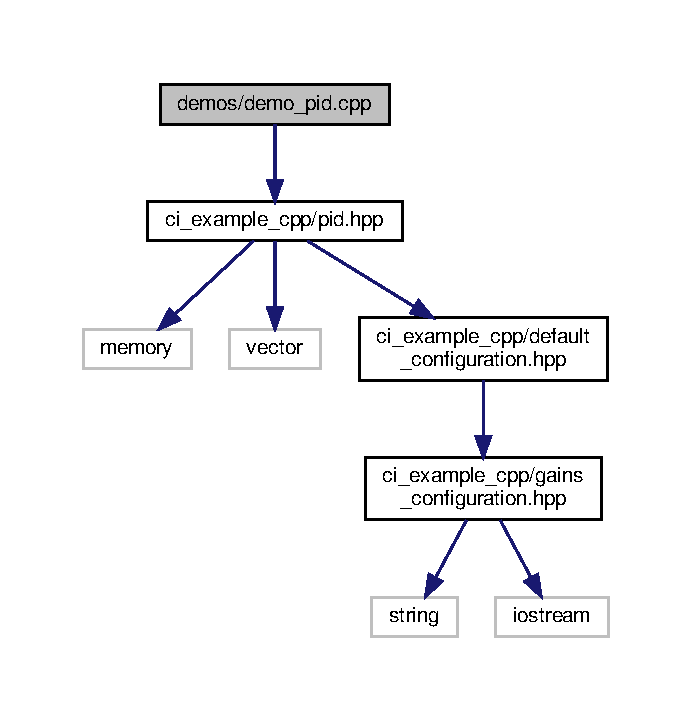
\includegraphics[width=332pt]{demo__pid_8cpp__incl}
\end{center}
\end{figure}
\subsection*{Functions}
\begin{DoxyCompactItemize}
\item 
\mbox{\Hypertarget{demo__pid_8cpp_aa5343637e5c7a19c19aae1beed976ab6}\label{demo__pid_8cpp_aa5343637e5c7a19c19aae1beed976ab6}} 
void \hyperlink{demo__pid_8cpp_aa5343637e5c7a19c19aae1beed976ab6}{run\+\_\+demo} ()
\begin{DoxyCompactList}\small\item\em Creates a P\+ID controller and use the A\+PI in a small demo. \end{DoxyCompactList}\item 
int \hyperlink{demo__pid_8cpp_ae66f6b31b5ad750f1fe042a706a4e3d4}{main} ()
\begin{DoxyCompactList}\small\item\em Execute the \hyperlink{demo__pid_8cpp_aa5343637e5c7a19c19aae1beed976ab6}{run\+\_\+demo()} trhough a try/catch expression. \end{DoxyCompactList}\end{DoxyCompactItemize}


\subsection{Detailed Description}
Example of a simple demo suitable for continuous integration. 

\begin{DoxyAuthor}{Author}
Vincent Berenz license License B\+S\+D-\/3-\/\+Clause 
\end{DoxyAuthor}
\begin{DoxyCopyright}{Copyright}
Copyright (c) 2019, New York University and Max Planck Gesellschaft. 
\end{DoxyCopyright}
\begin{DoxyDate}{Date}
2019-\/05-\/22
\end{DoxyDate}
\begin{DoxySeeAlso}{See also}
\href{https://git-amd.tuebingen.mpg.de/amd-clmc/ci_example/wikis/catkin:-how-to-implement-a-demo}{\tt https\+://git-\/amd.\+tuebingen.\+mpg.\+de/amd-\/clmc/ci\+\_\+example/wikis/catkin\+:-\/how-\/to-\/implement-\/a-\/demo} 
\end{DoxySeeAlso}


\subsection{Function Documentation}
\mbox{\Hypertarget{demo__pid_8cpp_ae66f6b31b5ad750f1fe042a706a4e3d4}\label{demo__pid_8cpp_ae66f6b31b5ad750f1fe042a706a4e3d4}} 
\index{demo\+\_\+pid.\+cpp@{demo\+\_\+pid.\+cpp}!main@{main}}
\index{main@{main}!demo\+\_\+pid.\+cpp@{demo\+\_\+pid.\+cpp}}
\subsubsection{\texorpdfstring{main()}{main()}}
{\footnotesize\ttfamily int main (\begin{DoxyParamCaption}{ }\end{DoxyParamCaption})}



Execute the \hyperlink{demo__pid_8cpp_aa5343637e5c7a19c19aae1beed976ab6}{run\+\_\+demo()} trhough a try/catch expression. 

\begin{DoxyReturn}{Returns}
int 
\end{DoxyReturn}
\begin{Desc}
\item[Examples\+: ]\par
\hyperlink{demo_pid_8cpp-example}{demo\+\_\+pid.\+cpp}.\end{Desc}

\hypertarget{demo__pid__load__from__file_8cpp}{}\section{demos/demo\+\_\+pid\+\_\+load\+\_\+from\+\_\+file.cpp File Reference}
\label{demo__pid__load__from__file_8cpp}\index{demos/demo\+\_\+pid\+\_\+load\+\_\+from\+\_\+file.\+cpp@{demos/demo\+\_\+pid\+\_\+load\+\_\+from\+\_\+file.\+cpp}}


Example of a demo that requires to read a config file.  


{\ttfamily \#include \char`\"{}ci\+\_\+example\+\_\+cpp/pid.\+hpp\char`\"{}}\newline
{\ttfamily \#include \char`\"{}ci\+\_\+example\+\_\+cpp/file\+\_\+configuration.\+hpp\char`\"{}}\newline
{\ttfamily \#include $<$stdexcept$>$}\newline
Include dependency graph for demo\+\_\+pid\+\_\+load\+\_\+from\+\_\+file.\+cpp\+:
\nopagebreak
\begin{figure}[H]
\begin{center}
\leavevmode
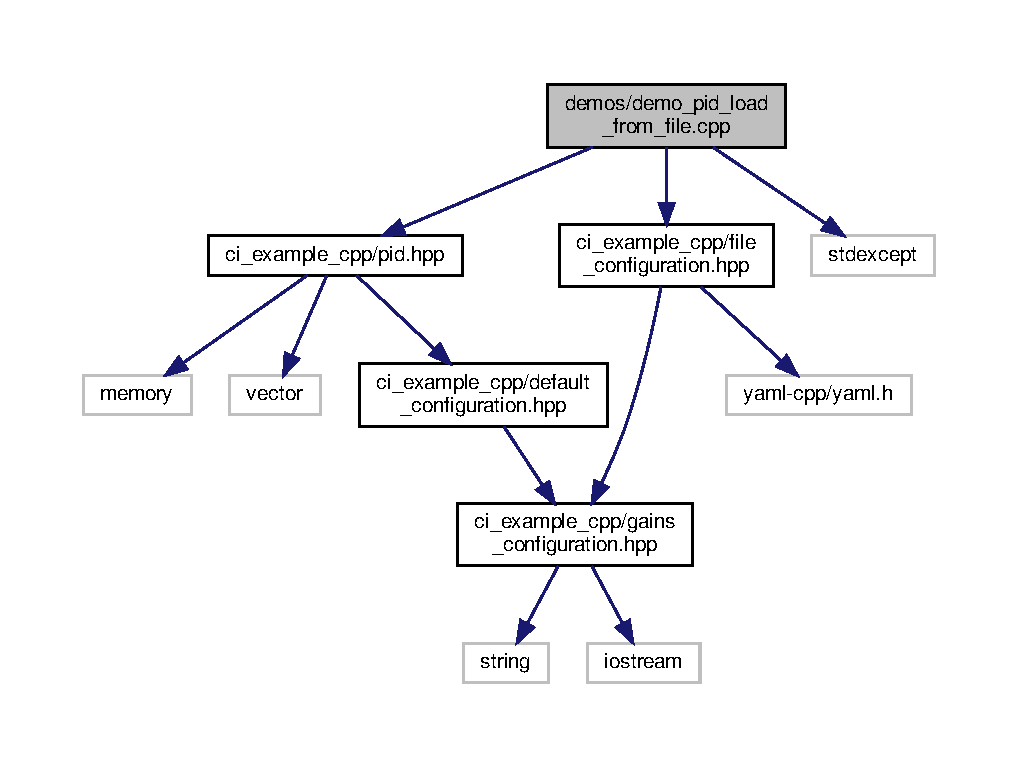
\includegraphics[width=350pt]{demo__pid__load__from__file_8cpp__incl}
\end{center}
\end{figure}
\subsection*{Functions}
\begin{DoxyCompactItemize}
\item 
\mbox{\Hypertarget{demo__pid__load__from__file_8cpp_aa5343637e5c7a19c19aae1beed976ab6}\label{demo__pid__load__from__file_8cpp_aa5343637e5c7a19c19aae1beed976ab6}} 
void \hyperlink{demo__pid__load__from__file_8cpp_aa5343637e5c7a19c19aae1beed976ab6}{run\+\_\+demo} ()
\begin{DoxyCompactList}\small\item\em Run some demo using a Y\+A\+ML file as configuration for the P\+ID controller. \end{DoxyCompactList}\item 
\mbox{\Hypertarget{demo__pid__load__from__file_8cpp_ae66f6b31b5ad750f1fe042a706a4e3d4}\label{demo__pid__load__from__file_8cpp_ae66f6b31b5ad750f1fe042a706a4e3d4}} 
int \hyperlink{demo__pid__load__from__file_8cpp_ae66f6b31b5ad750f1fe042a706a4e3d4}{main} ()
\begin{DoxyCompactList}\small\item\em Run the demo in a safe environment. \end{DoxyCompactList}\end{DoxyCompactItemize}


\subsection{Detailed Description}
Example of a demo that requires to read a config file. 

\begin{DoxyAuthor}{Author}
Vincent Berenz license License B\+S\+D-\/3-\/\+Clause 
\end{DoxyAuthor}
\begin{DoxyCopyright}{Copyright}
Copyright (c) 2019, New York University and Max Planck Gesellschaft. 
\end{DoxyCopyright}
\begin{DoxyDate}{Date}
2019-\/05-\/22
\end{DoxyDate}
\begin{DoxySeeAlso}{See also}
\href{https://git-amd.tuebingen.mpg.de/amd-clmc/ci_example/wikis/catkin:-how-to-implement-a-demo}{\tt https\+://git-\/amd.\+tuebingen.\+mpg.\+de/amd-\/clmc/ci\+\_\+example/wikis/catkin\+:-\/how-\/to-\/implement-\/a-\/demo} 
\end{DoxySeeAlso}

\hypertarget{default__configuration_8hpp}{}\section{include/ci\+\_\+example\+\_\+cpp/default\+\_\+configuration.hpp File Reference}
\label{default__configuration_8hpp}\index{include/ci\+\_\+example\+\_\+cpp/default\+\_\+configuration.\+hpp@{include/ci\+\_\+example\+\_\+cpp/default\+\_\+configuration.\+hpp}}
{\ttfamily \#include \char`\"{}ci\+\_\+example\+\_\+cpp/gains\+\_\+configuration.\+hpp\char`\"{}}\newline
Include dependency graph for default\+\_\+configuration.\+hpp\+:
\nopagebreak
\begin{figure}[H]
\begin{center}
\leavevmode
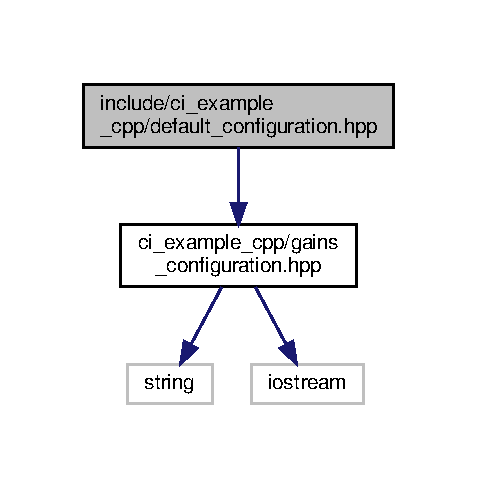
\includegraphics[width=229pt]{default__configuration_8hpp__incl}
\end{center}
\end{figure}
This graph shows which files directly or indirectly include this file\+:
\nopagebreak
\begin{figure}[H]
\begin{center}
\leavevmode
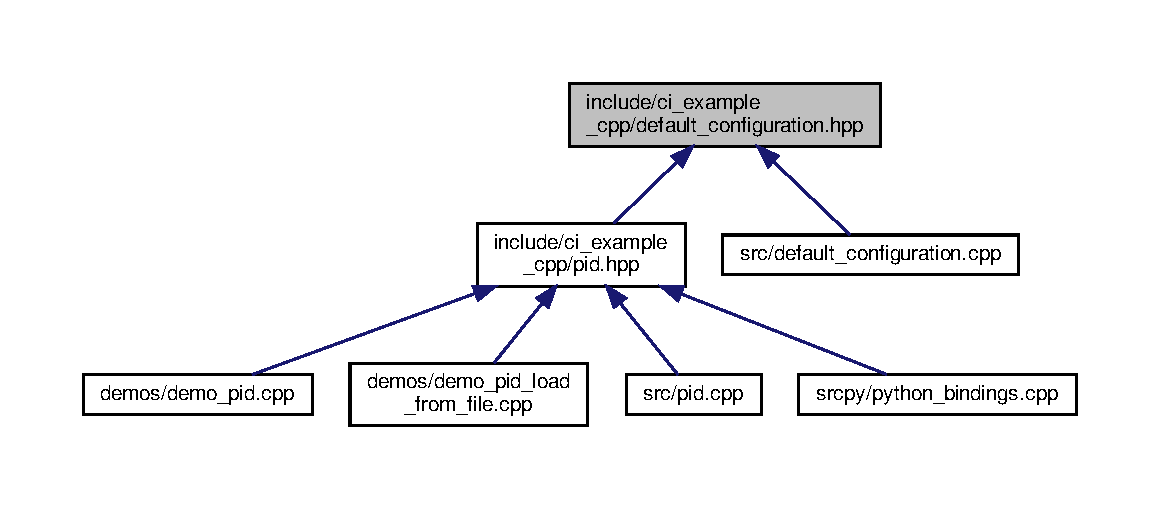
\includegraphics[width=350pt]{default__configuration_8hpp__dep__incl}
\end{center}
\end{figure}
\subsection*{Classes}
\begin{DoxyCompactItemize}
\item 
class \hyperlink{classci__example__cpp_1_1DefaultConfiguration}{ci\+\_\+example\+\_\+cpp\+::\+Default\+Configuration}
\begin{DoxyCompactList}\small\item\em Default configuration for the kp, kd, ki paramters. \end{DoxyCompactList}\end{DoxyCompactItemize}
\subsection*{Macros}
\begin{DoxyCompactItemize}
\item 
\mbox{\Hypertarget{default__configuration_8hpp_a0a0faa44632edd1da90cf562ec2f19e6}\label{default__configuration_8hpp_a0a0faa44632edd1da90cf562ec2f19e6}} 
\#define {\bfseries D\+E\+F\+A\+U\+L\+T\+\_\+\+KP}~1.\+0
\item 
\mbox{\Hypertarget{default__configuration_8hpp_a133d0d1f063256087b0f0dde400926a6}\label{default__configuration_8hpp_a133d0d1f063256087b0f0dde400926a6}} 
\#define {\bfseries D\+E\+F\+A\+U\+L\+T\+\_\+\+KD}~1.\+0
\item 
\mbox{\Hypertarget{default__configuration_8hpp_a4567b54152d2a9baae45716e3ab66d7c}\label{default__configuration_8hpp_a4567b54152d2a9baae45716e3ab66d7c}} 
\#define {\bfseries D\+E\+F\+A\+U\+L\+T\+\_\+\+KI}~1.\+0
\end{DoxyCompactItemize}


\subsection{Detailed Description}
\begin{DoxyAuthor}{Author}
Vincent Berenz 
\end{DoxyAuthor}
\begin{DoxyCopyright}{Copyright}
Copyright (c) 2019, New York University and Max Planck Gesellschaft, License B\+S\+D-\/3-\/\+Clause 
\end{DoxyCopyright}
\begin{DoxyDate}{Date}
2019-\/12-\/09 
\end{DoxyDate}

\hypertarget{file__configuration_8hpp}{}\section{include/ci\+\_\+example\+\_\+cpp/file\+\_\+configuration.hpp File Reference}
\label{file__configuration_8hpp}\index{include/ci\+\_\+example\+\_\+cpp/file\+\_\+configuration.\+hpp@{include/ci\+\_\+example\+\_\+cpp/file\+\_\+configuration.\+hpp}}
{\ttfamily \#include \char`\"{}yaml-\/cpp/yaml.\+h\char`\"{}}\newline
{\ttfamily \#include \char`\"{}ci\+\_\+example\+\_\+cpp/gains\+\_\+configuration.\+hpp\char`\"{}}\newline
Include dependency graph for file\+\_\+configuration.\+hpp\+:
\nopagebreak
\begin{figure}[H]
\begin{center}
\leavevmode
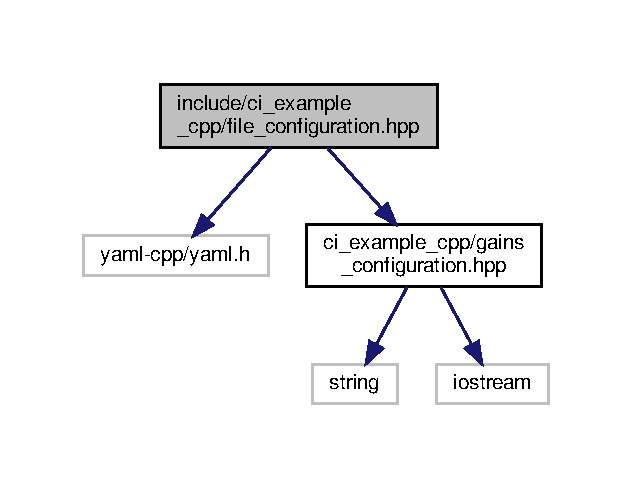
\includegraphics[width=304pt]{file__configuration_8hpp__incl}
\end{center}
\end{figure}
This graph shows which files directly or indirectly include this file\+:
\nopagebreak
\begin{figure}[H]
\begin{center}
\leavevmode
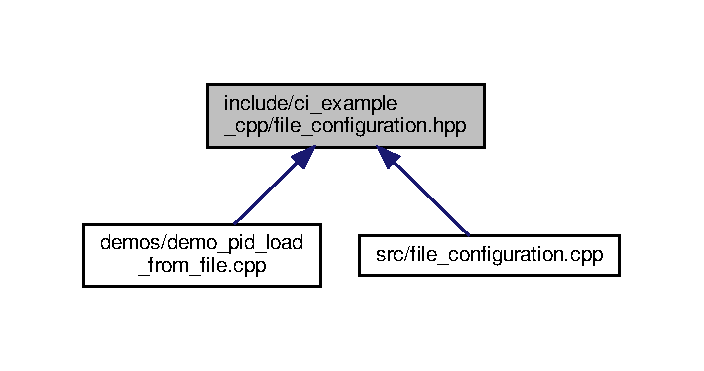
\includegraphics[width=338pt]{file__configuration_8hpp__dep__incl}
\end{center}
\end{figure}
\subsection*{Classes}
\begin{DoxyCompactItemize}
\item 
class \hyperlink{classci__example__cpp_1_1File__configuration}{ci\+\_\+example\+\_\+cpp\+::\+File\+\_\+configuration}
\begin{DoxyCompactList}\small\item\em Reading configuration from yaml file. \end{DoxyCompactList}\end{DoxyCompactItemize}


\subsection{Detailed Description}
\begin{DoxyAuthor}{Author}
Vincent Berenz 
\end{DoxyAuthor}
\begin{DoxyCopyright}{Copyright}
Copyright (c) 2019, New York University and Max Planck Gesellschaft, License B\+S\+D-\/3-\/\+Clause 
\end{DoxyCopyright}
\begin{DoxyDate}{Date}
2019-\/12-\/09 
\end{DoxyDate}

\hypertarget{gains__configuration_8hpp}{}\section{include/ci\+\_\+example\+\_\+cpp/gains\+\_\+configuration.hpp File Reference}
\label{gains__configuration_8hpp}\index{include/ci\+\_\+example\+\_\+cpp/gains\+\_\+configuration.\+hpp@{include/ci\+\_\+example\+\_\+cpp/gains\+\_\+configuration.\+hpp}}
{\ttfamily \#include $<$string$>$}\newline
{\ttfamily \#include $<$iostream$>$}\newline
Include dependency graph for gains\+\_\+configuration.\+hpp\+:
\nopagebreak
\begin{figure}[H]
\begin{center}
\leavevmode
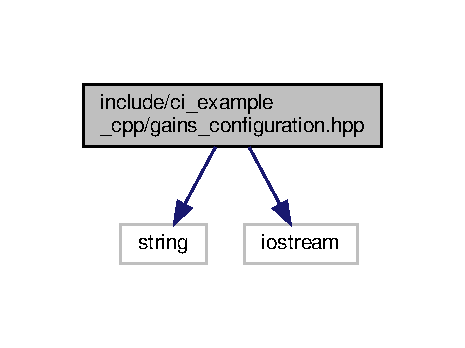
\includegraphics[width=223pt]{gains__configuration_8hpp__incl}
\end{center}
\end{figure}
This graph shows which files directly or indirectly include this file\+:
\nopagebreak
\begin{figure}[H]
\begin{center}
\leavevmode
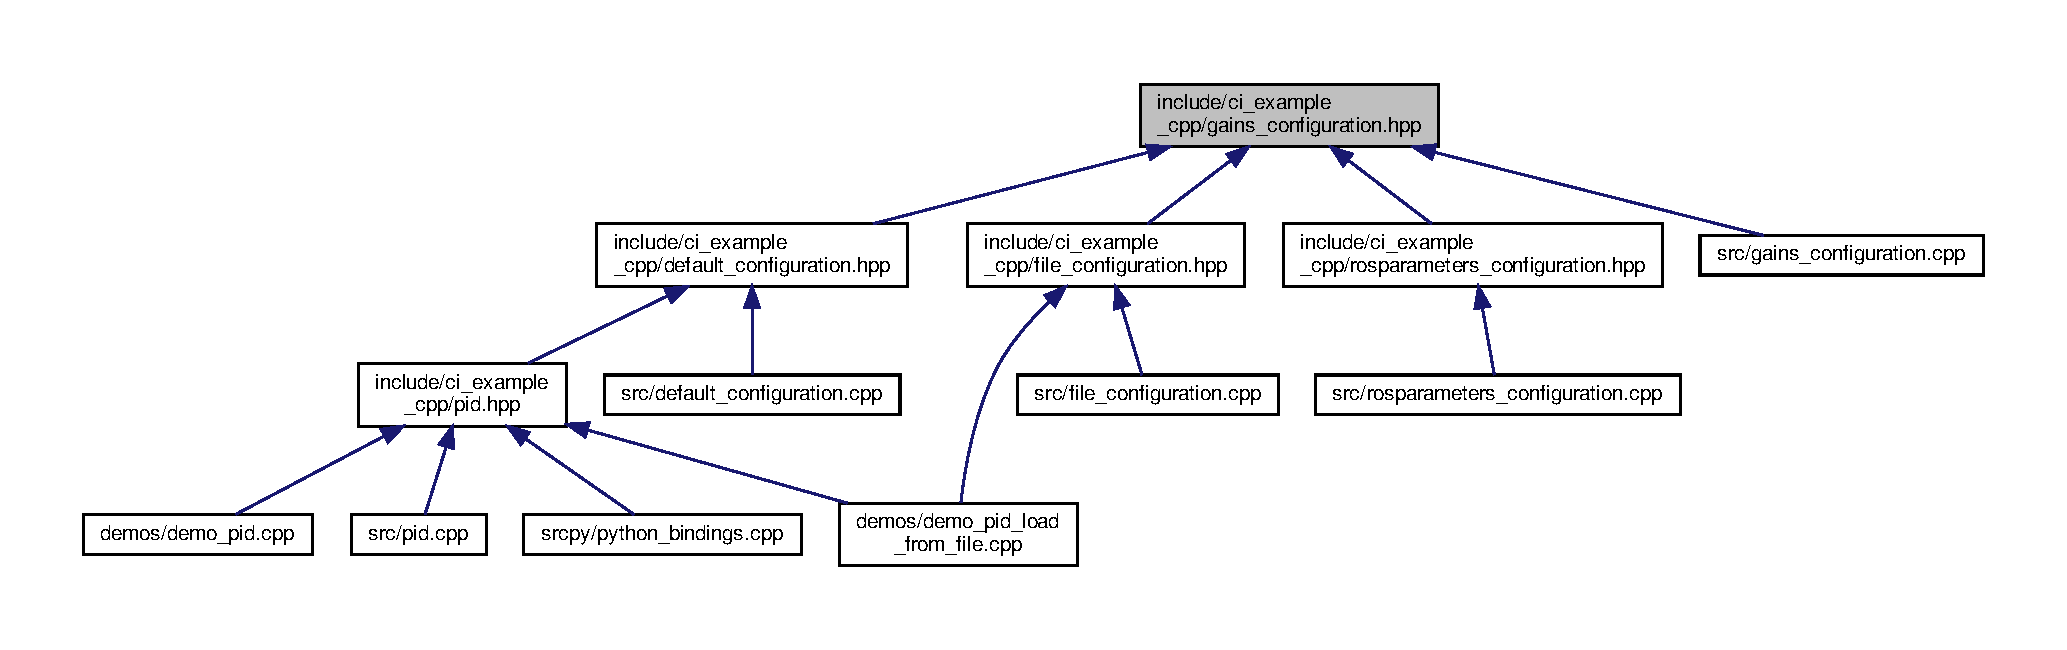
\includegraphics[width=350pt]{gains__configuration_8hpp__dep__incl}
\end{center}
\end{figure}
\subsection*{Classes}
\begin{DoxyCompactItemize}
\item 
class \hyperlink{classci__example__cpp_1_1Gains__configuration}{ci\+\_\+example\+\_\+cpp\+::\+Gains\+\_\+configuration}
\begin{DoxyCompactList}\small\item\em Abstract class defining for the \hyperlink{classci__example__cpp_1_1PID}{P\+ID} configuration. \end{DoxyCompactList}\end{DoxyCompactItemize}
\subsection*{Functions}
\begin{DoxyCompactItemize}
\item 
void \hyperlink{gains__configuration_8hpp_a2400ff05e31dee6aced75d9c230b9fe5}{ci\+\_\+example\+\_\+cpp\+::print\+\_\+configuration} (const Gains\+\_\+configuration \&configuration)
\end{DoxyCompactItemize}


\subsection{Detailed Description}
\begin{DoxyAuthor}{Author}
Vincent Berenz 
\end{DoxyAuthor}
\begin{DoxyCopyright}{Copyright}
Copyright (c) 2019, New York University and Max Planck Gesellschaft, License B\+S\+D-\/3-\/\+Clause 
\end{DoxyCopyright}
\begin{DoxyDate}{Date}
2019-\/12-\/09 
\end{DoxyDate}


\subsection{Function Documentation}
\mbox{\Hypertarget{gains__configuration_8hpp_file_a2400ff05e31dee6aced75d9c230b9fe5}\label{gains__configuration_8hpp_file_a2400ff05e31dee6aced75d9c230b9fe5}} 
\index{gains\+\_\+configuration.\+hpp@{gains\+\_\+configuration.\+hpp}!print\+\_\+configuration@{print\+\_\+configuration}}
\index{print\+\_\+configuration@{print\+\_\+configuration}!gains\+\_\+configuration.\+hpp@{gains\+\_\+configuration.\+hpp}}
\subsubsection{\texorpdfstring{print\+\_\+configuration()}{print\_configuration()}}
{\footnotesize\ttfamily void ci\+\_\+example\+\_\+cpp\+::print\+\_\+configuration (\begin{DoxyParamCaption}\item[{const \hyperlink{classci__example__cpp_1_1Gains__configuration}{Gains\+\_\+configuration} \&}]{configuration }\end{DoxyParamCaption})}

print values encapsulated by the provided configuration console on the standard output \begin{Desc}
\item[Examples\+: ]\par
\hyperlink{demo_pid_load_from_file_8cpp-example}{demo\+\_\+pid\+\_\+load\+\_\+from\+\_\+file.\+cpp}.\end{Desc}

\hypertarget{pid_8hpp}{}\section{include/ci\+\_\+example\+\_\+cpp/pid.hpp File Reference}
\label{pid_8hpp}\index{include/ci\+\_\+example\+\_\+cpp/pid.\+hpp@{include/ci\+\_\+example\+\_\+cpp/pid.\+hpp}}
{\ttfamily \#include $<$memory$>$}\newline
{\ttfamily \#include $<$vector$>$}\newline
{\ttfamily \#include \char`\"{}ci\+\_\+example\+\_\+cpp/default\+\_\+configuration.\+hpp\char`\"{}}\newline
Include dependency graph for pid.\+hpp\+:
\nopagebreak
\begin{figure}[H]
\begin{center}
\leavevmode
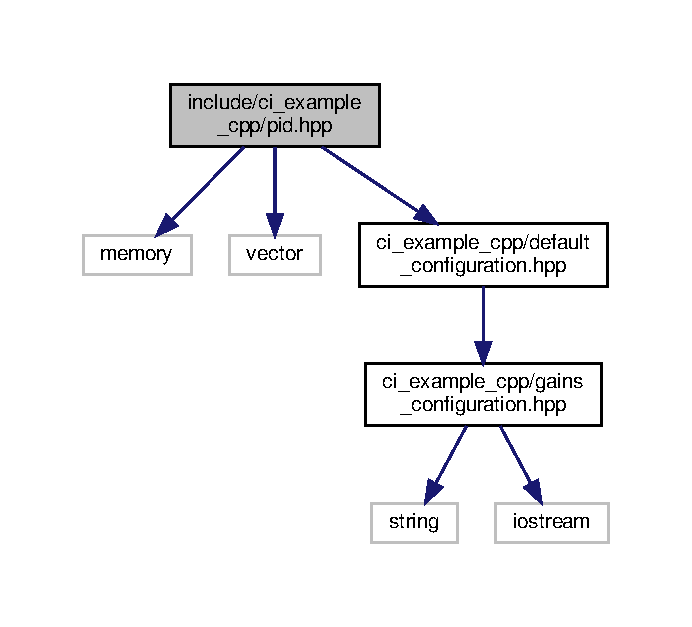
\includegraphics[width=332pt]{pid_8hpp__incl}
\end{center}
\end{figure}
This graph shows which files directly or indirectly include this file\+:
\nopagebreak
\begin{figure}[H]
\begin{center}
\leavevmode
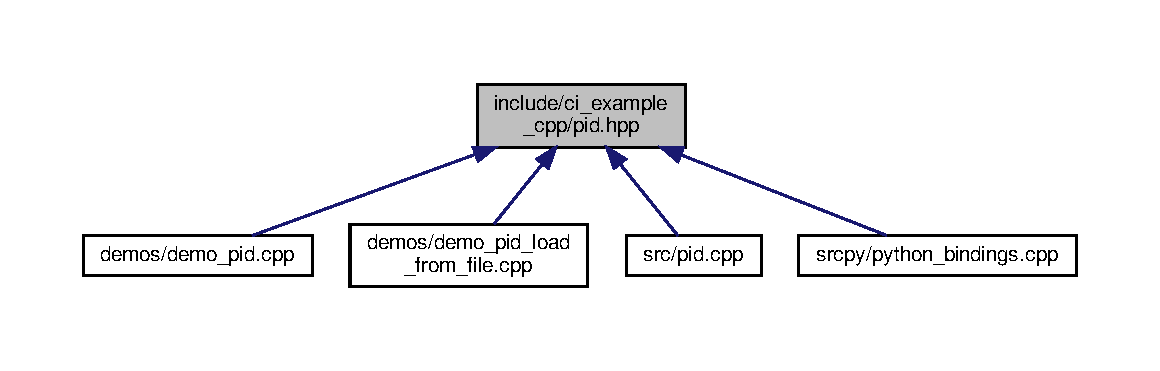
\includegraphics[width=350pt]{pid_8hpp__dep__incl}
\end{center}
\end{figure}
\subsection*{Classes}
\begin{DoxyCompactItemize}
\item 
class \hyperlink{classci__example__cpp_1_1PID}{ci\+\_\+example\+\_\+cpp\+::\+P\+ID}
\begin{DoxyCompactList}\small\item\em Simple 1D pid controller. \end{DoxyCompactList}\end{DoxyCompactItemize}
\subsection*{Functions}
\begin{DoxyCompactItemize}
\item 
P\+ID \& \hyperlink{pid_8hpp_ae98dfa6f474e368f3d1865d65406ec1f}{ci\+\_\+example\+\_\+cpp\+::get\+\_\+default\+\_\+pid} ()
\begin{DoxyCompactList}\small\item\em convenience factory for getting default controller, i.\+e. \end{DoxyCompactList}\end{DoxyCompactItemize}


\subsection{Detailed Description}
\begin{DoxyAuthor}{Author}
Vincent Berenz 
\end{DoxyAuthor}
\begin{DoxyCopyright}{Copyright}
Copyright (c) 2019, New York University and Max Planck Gesellschaft, License B\+S\+D-\/3-\/\+Clause 
\end{DoxyCopyright}
\begin{DoxyDate}{Date}
2019-\/12-\/09 
\end{DoxyDate}


\subsection{Function Documentation}
\mbox{\Hypertarget{pid_8hpp_file_ae98dfa6f474e368f3d1865d65406ec1f}\label{pid_8hpp_file_ae98dfa6f474e368f3d1865d65406ec1f}} 
\index{pid.\+hpp@{pid.\+hpp}!get\+\_\+default\+\_\+pid@{get\+\_\+default\+\_\+pid}}
\index{get\+\_\+default\+\_\+pid@{get\+\_\+default\+\_\+pid}!pid.\+hpp@{pid.\+hpp}}
\subsubsection{\texorpdfstring{get\+\_\+default\+\_\+pid()}{get\_default\_pid()}}
{\footnotesize\ttfamily P\+ID \& ci\+\_\+example\+\_\+cpp\+::get\+\_\+default\+\_\+pid (\begin{DoxyParamCaption}{ }\end{DoxyParamCaption})}



convenience factory for getting default controller, i.\+e. 

same as P\+I\+D(std\+::shared\+\_\+ptr$<$\+Default\+Configuration$>$ configuration) \begin{DoxySeeAlso}{See also}
Default\+Configuration 
\end{DoxySeeAlso}
\begin{Desc}
\item[Examples\+: ]\par
\hyperlink{demo_pid_8cpp-example}{demo\+\_\+pid.\+cpp}.\end{Desc}

\hypertarget{rosparameters__configuration_8hpp}{}\section{include/ci\+\_\+example\+\_\+cpp/rosparameters\+\_\+configuration.hpp File Reference}
\label{rosparameters__configuration_8hpp}\index{include/ci\+\_\+example\+\_\+cpp/rosparameters\+\_\+configuration.\+hpp@{include/ci\+\_\+example\+\_\+cpp/rosparameters\+\_\+configuration.\+hpp}}
{\ttfamily \#include \char`\"{}ros/ros.\+h\char`\"{}}\newline
{\ttfamily \#include \char`\"{}ros/master.\+h\char`\"{}}\newline
{\ttfamily \#include \char`\"{}ci\+\_\+example\+\_\+cpp/gains\+\_\+configuration.\+hpp\char`\"{}}\newline
Include dependency graph for rosparameters\+\_\+configuration.\+hpp\+:
\nopagebreak
\begin{figure}[H]
\begin{center}
\leavevmode
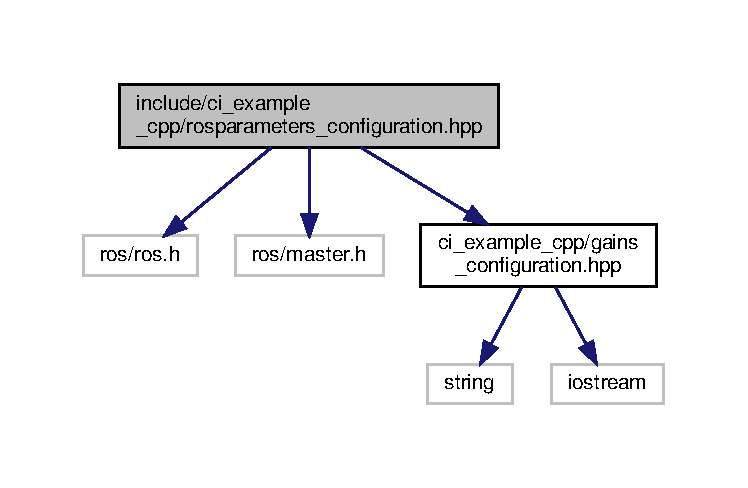
\includegraphics[width=350pt]{rosparameters__configuration_8hpp__incl}
\end{center}
\end{figure}
This graph shows which files directly or indirectly include this file\+:
\nopagebreak
\begin{figure}[H]
\begin{center}
\leavevmode
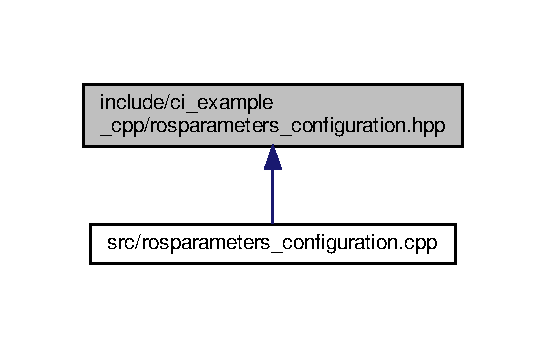
\includegraphics[width=262pt]{rosparameters__configuration_8hpp__dep__incl}
\end{center}
\end{figure}
\subsection*{Classes}
\begin{DoxyCompactItemize}
\item 
class \hyperlink{classci__example__cpp_1_1RosParameters__configuration}{ci\+\_\+example\+\_\+cpp\+::\+Ros\+Parameters\+\_\+configuration}
\begin{DoxyCompactList}\small\item\em Read gains configuration from the ros parameter server. \end{DoxyCompactList}\end{DoxyCompactItemize}
\subsection*{Macros}
\begin{DoxyCompactItemize}
\item 
\mbox{\Hypertarget{rosparameters__configuration_8hpp_af16e459619ed78c40f8aaacb1689d2f1}\label{rosparameters__configuration_8hpp_af16e459619ed78c40f8aaacb1689d2f1}} 
\#define {\bfseries R\+O\+S\+P\+A\+R\+A\+M\+\_\+\+KP}~\char`\"{}gains\+\_\+kp\char`\"{}
\item 
\mbox{\Hypertarget{rosparameters__configuration_8hpp_a3eb612796d47d8091761995b9f1b05de}\label{rosparameters__configuration_8hpp_a3eb612796d47d8091761995b9f1b05de}} 
\#define {\bfseries R\+O\+S\+P\+A\+R\+A\+M\+\_\+\+KD}~\char`\"{}gains\+\_\+kd\char`\"{}
\item 
\mbox{\Hypertarget{rosparameters__configuration_8hpp_a6537ebe35c054740ab6578e12266564c}\label{rosparameters__configuration_8hpp_a6537ebe35c054740ab6578e12266564c}} 
\#define {\bfseries R\+O\+S\+P\+A\+R\+A\+M\+\_\+\+KI}~\char`\"{}gains\+\_\+ki\char`\"{}
\end{DoxyCompactItemize}


\subsection{Detailed Description}
\begin{DoxyAuthor}{Author}
Vincent Berenz 
\end{DoxyAuthor}
\begin{DoxyCopyright}{Copyright}
Copyright (c) 2019, New York University and Max Planck Gesellschaft, License B\+S\+D-\/3-\/\+Clause 
\end{DoxyCopyright}
\begin{DoxyDate}{Date}
2019-\/12-\/09 
\end{DoxyDate}

\hypertarget{basic__pid_8cpp}{}\section{src/basic\+\_\+pid.cpp File Reference}
\label{basic__pid_8cpp}\index{src/basic\+\_\+pid.\+cpp@{src/basic\+\_\+pid.\+cpp}}
{\ttfamily \#include \char`\"{}ci\+\_\+example\+\_\+cpp/basic\+\_\+pid.\+hpp\char`\"{}}\newline
Include dependency graph for basic\+\_\+pid.\+cpp\+:
\nopagebreak
\begin{figure}[H]
\begin{center}
\leavevmode
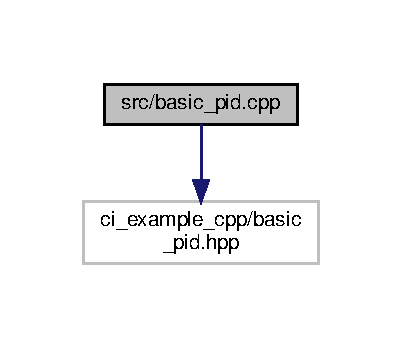
\includegraphics[width=193pt]{basic__pid_8cpp__incl}
\end{center}
\end{figure}


\subsection{Detailed Description}
\begin{DoxyAuthor}{Author}
Vincent Berenz license License B\+S\+D-\/3-\/\+Clause 
\end{DoxyAuthor}
\begin{DoxyCopyright}{Copyright}
Copyright (c) 2019, New York University and Max Planck Gesellschaft. 
\end{DoxyCopyright}
\begin{DoxyDate}{Date}
2019-\/05-\/22 
\end{DoxyDate}

\hypertarget{default__configuration_8cpp}{}\section{src/default\+\_\+configuration.cpp File Reference}
\label{default__configuration_8cpp}\index{src/default\+\_\+configuration.\+cpp@{src/default\+\_\+configuration.\+cpp}}
{\ttfamily \#include \char`\"{}ci\+\_\+example\+\_\+cpp/default\+\_\+configuration.\+hpp\char`\"{}}\newline
Include dependency graph for default\+\_\+configuration.\+cpp\+:
\nopagebreak
\begin{figure}[H]
\begin{center}
\leavevmode
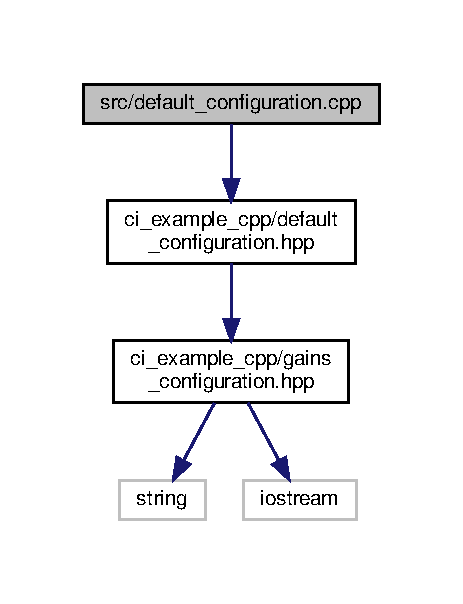
\includegraphics[width=222pt]{default__configuration_8cpp__incl}
\end{center}
\end{figure}


\subsection{Detailed Description}
\begin{DoxyAuthor}{Author}
Vincent Berenz 
\end{DoxyAuthor}
\begin{DoxyCopyright}{Copyright}
Copyright (c) 2019, New York University and Max Planck Gesellschaft, License B\+S\+D-\/3-\/\+Clause 
\end{DoxyCopyright}
\begin{DoxyDate}{Date}
2019-\/12-\/09 
\end{DoxyDate}

\hypertarget{file__configuration_8cpp}{}\section{src/file\+\_\+configuration.cpp File Reference}
\label{file__configuration_8cpp}\index{src/file\+\_\+configuration.\+cpp@{src/file\+\_\+configuration.\+cpp}}
{\ttfamily \#include \char`\"{}ci\+\_\+example\+\_\+cpp/file\+\_\+configuration.\+hpp\char`\"{}}\newline
Include dependency graph for file\+\_\+configuration.\+cpp\+:
\nopagebreak
\begin{figure}[H]
\begin{center}
\leavevmode
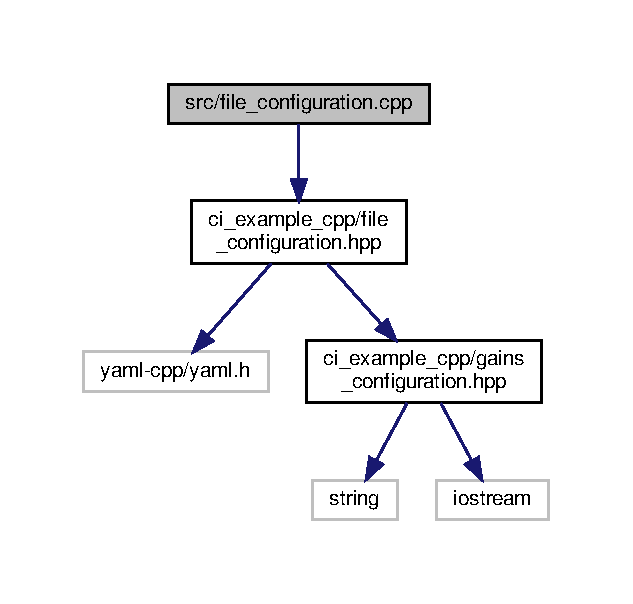
\includegraphics[width=304pt]{file__configuration_8cpp__incl}
\end{center}
\end{figure}


\subsection{Detailed Description}
\begin{DoxyAuthor}{Author}
Vincent Berenz 
\end{DoxyAuthor}
\begin{DoxyCopyright}{Copyright}
Copyright (c) 2019, New York University and Max Planck Gesellschaft, License B\+S\+D-\/3-\/\+Clause 
\end{DoxyCopyright}
\begin{DoxyDate}{Date}
2019-\/12-\/09 
\end{DoxyDate}

\hypertarget{gains__configuration_8cpp}{}\section{src/gains\+\_\+configuration.cpp File Reference}
\label{gains__configuration_8cpp}\index{src/gains\+\_\+configuration.\+cpp@{src/gains\+\_\+configuration.\+cpp}}
{\ttfamily \#include \char`\"{}ci\+\_\+example\+\_\+cpp/gains\+\_\+configuration.\+hpp\char`\"{}}\newline
Include dependency graph for gains\+\_\+configuration.\+cpp\+:
\nopagebreak
\begin{figure}[H]
\begin{center}
\leavevmode
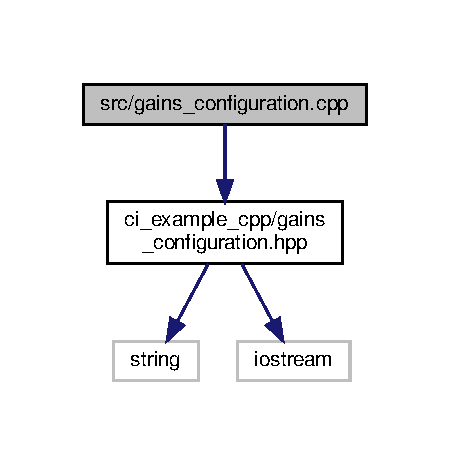
\includegraphics[width=216pt]{gains__configuration_8cpp__incl}
\end{center}
\end{figure}
\subsection*{Functions}
\begin{DoxyCompactItemize}
\item 
void \hyperlink{gains__configuration_8hpp_a2400ff05e31dee6aced75d9c230b9fe5}{ci\+\_\+example\+\_\+cpp\+::print\+\_\+configuration} (const Gains\+\_\+configuration \&configuration)
\end{DoxyCompactItemize}


\subsection{Detailed Description}
\begin{DoxyAuthor}{Author}
Vincent Berenz 
\end{DoxyAuthor}
\begin{DoxyCopyright}{Copyright}
Copyright (c) 2019, New York University and Max Planck Gesellschaft, License B\+S\+D-\/3-\/\+Clause 
\end{DoxyCopyright}
\begin{DoxyDate}{Date}
2019-\/12-\/09 
\end{DoxyDate}


\subsection{Function Documentation}
\mbox{\Hypertarget{gains__configuration_8hpp_file_a2400ff05e31dee6aced75d9c230b9fe5}\label{gains__configuration_8hpp_file_a2400ff05e31dee6aced75d9c230b9fe5}} 
\index{gains\+\_\+configuration.\+cpp@{gains\+\_\+configuration.\+cpp}!print\+\_\+configuration@{print\+\_\+configuration}}
\index{print\+\_\+configuration@{print\+\_\+configuration}!gains\+\_\+configuration.\+cpp@{gains\+\_\+configuration.\+cpp}}
\subsubsection{\texorpdfstring{print\+\_\+configuration()}{print\_configuration()}}
{\footnotesize\ttfamily void ci\+\_\+example\+\_\+cpp\+::print\+\_\+configuration (\begin{DoxyParamCaption}\item[{const \hyperlink{classci__example__cpp_1_1Gains__configuration}{Gains\+\_\+configuration} \&}]{configuration }\end{DoxyParamCaption})}

print values encapsulated by the provided configuration console on the standard output \begin{Desc}
\item[Examples\+: ]\par
\hyperlink{demo_pid_load_from_file_8cpp-example}{demo\+\_\+pid\+\_\+load\+\_\+from\+\_\+file.\+cpp}.\end{Desc}

\hypertarget{pid_8cpp}{}\section{src/pid.cpp File Reference}
\label{pid_8cpp}\index{src/pid.\+cpp@{src/pid.\+cpp}}
{\ttfamily \#include \char`\"{}ci\+\_\+example\+\_\+cpp/pid.\+hpp\char`\"{}}\newline
Include dependency graph for pid.\+cpp\+:
\nopagebreak
\begin{figure}[H]
\begin{center}
\leavevmode
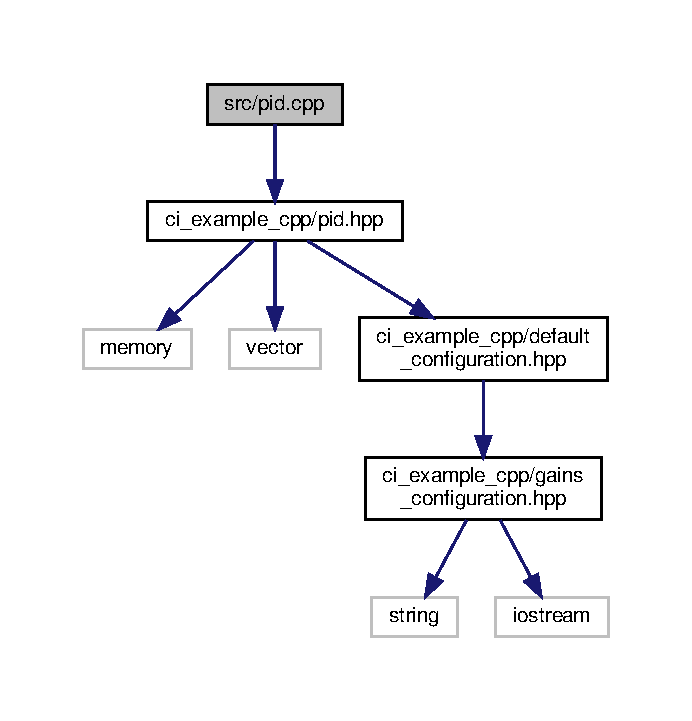
\includegraphics[width=332pt]{pid_8cpp__incl}
\end{center}
\end{figure}
\subsection*{Classes}
\begin{DoxyCompactItemize}
\item 
class \hyperlink{classci__example__cpp_1_1Default__pid__factory}{ci\+\_\+example\+\_\+cpp\+::\+Default\+\_\+pid\+\_\+factory}
\begin{DoxyCompactList}\small\item\em Use a \hyperlink{classci__example__cpp_1_1PID}{P\+ID} factory for the unittests. \end{DoxyCompactList}\end{DoxyCompactItemize}
\subsection*{Functions}
\begin{DoxyCompactItemize}
\item 
P\+ID \& \hyperlink{pid_8hpp_ae98dfa6f474e368f3d1865d65406ec1f}{ci\+\_\+example\+\_\+cpp\+::get\+\_\+default\+\_\+pid} ()
\begin{DoxyCompactList}\small\item\em convenience factory for getting default controller, i.\+e. \end{DoxyCompactList}\end{DoxyCompactItemize}


\subsection{Detailed Description}
\begin{DoxyAuthor}{Author}
Vincent Berenz 
\end{DoxyAuthor}
\begin{DoxyCopyright}{Copyright}
Copyright (c) 2019, New York University and Max Planck Gesellschaft, License B\+S\+D-\/3-\/\+Clause 
\end{DoxyCopyright}
\begin{DoxyDate}{Date}
2019-\/12-\/09 
\end{DoxyDate}


\subsection{Function Documentation}
\mbox{\Hypertarget{pid_8hpp_file_ae98dfa6f474e368f3d1865d65406ec1f}\label{pid_8hpp_file_ae98dfa6f474e368f3d1865d65406ec1f}} 
\index{pid.\+cpp@{pid.\+cpp}!get\+\_\+default\+\_\+pid@{get\+\_\+default\+\_\+pid}}
\index{get\+\_\+default\+\_\+pid@{get\+\_\+default\+\_\+pid}!pid.\+cpp@{pid.\+cpp}}
\subsubsection{\texorpdfstring{get\+\_\+default\+\_\+pid()}{get\_default\_pid()}}
{\footnotesize\ttfamily P\+ID \& ci\+\_\+example\+\_\+cpp\+::get\+\_\+default\+\_\+pid (\begin{DoxyParamCaption}{ }\end{DoxyParamCaption})}



convenience factory for getting default controller, i.\+e. 

same as P\+I\+D(std\+::shared\+\_\+ptr$<$\+Default\+Configuration$>$ configuration) \begin{DoxySeeAlso}{See also}
Default\+Configuration 
\end{DoxySeeAlso}
\begin{Desc}
\item[Examples\+: ]\par
\hyperlink{demo_pid_8cpp-example}{demo\+\_\+pid.\+cpp}.\end{Desc}

\hypertarget{rosparameters__configuration_8cpp}{}\section{src/rosparameters\+\_\+configuration.cpp File Reference}
\label{rosparameters__configuration_8cpp}\index{src/rosparameters\+\_\+configuration.\+cpp@{src/rosparameters\+\_\+configuration.\+cpp}}
{\ttfamily \#include \char`\"{}ci\+\_\+example\+\_\+cpp/rosparameters\+\_\+configuration.\+hpp\char`\"{}}\newline
Include dependency graph for rosparameters\+\_\+configuration.\+cpp\+:
\nopagebreak
\begin{figure}[H]
\begin{center}
\leavevmode
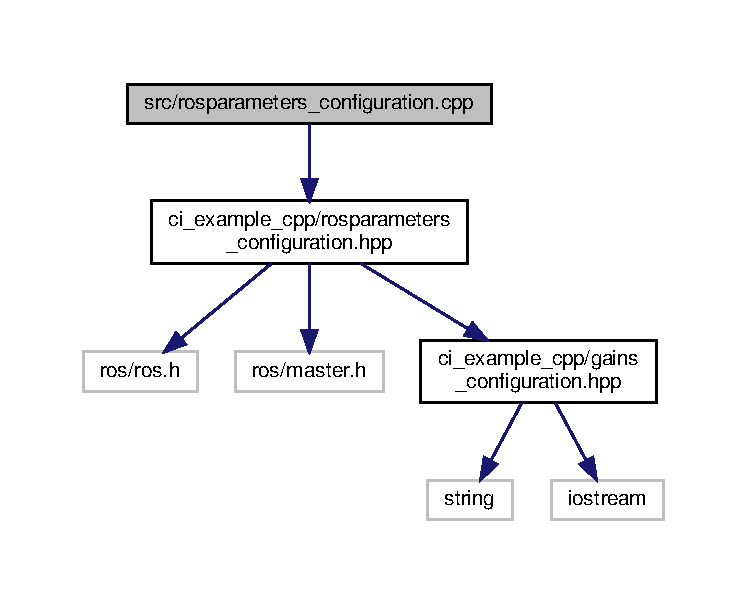
\includegraphics[width=350pt]{rosparameters__configuration_8cpp__incl}
\end{center}
\end{figure}
\subsection*{Functions}
\begin{DoxyCompactItemize}
\item 
\mbox{\Hypertarget{rosparameters__configuration_8cpp_a2f348a20def1e6740ec6edc67860bd60}\label{rosparameters__configuration_8cpp_a2f348a20def1e6740ec6edc67860bd60}} 
static bool {\bfseries ci\+\_\+example\+\_\+cpp\+::get\+\_\+parameter} (const ros\+::\+Node\+Handle \&nh, const std\+::string \&parameter, double \&get\+\_\+value)
\end{DoxyCompactItemize}


\subsection{Detailed Description}
\begin{DoxyAuthor}{Author}
Vincent Berenz 
\end{DoxyAuthor}
\begin{DoxyCopyright}{Copyright}
Copyright (c) 2019, New York University and Max Planck Gesellschaft, License B\+S\+D-\/3-\/\+Clause 
\end{DoxyCopyright}
\begin{DoxyDate}{Date}
2019-\/12-\/09 
\end{DoxyDate}

\hypertarget{python__bindings_8cpp}{}\section{srcpy/python\+\_\+bindings.cpp File Reference}
\label{python__bindings_8cpp}\index{srcpy/python\+\_\+bindings.\+cpp@{srcpy/python\+\_\+bindings.\+cpp}}


license License B\+S\+D-\/3-\/\+Clause  


{\ttfamily \#include $<$pybind11/pybind11.\+h$>$}\newline
{\ttfamily \#include \char`\"{}ci\+\_\+example\+\_\+cpp/pid.\+hpp\char`\"{}}\newline
Include dependency graph for python\+\_\+bindings.\+cpp\+:
\nopagebreak
\begin{figure}[H]
\begin{center}
\leavevmode
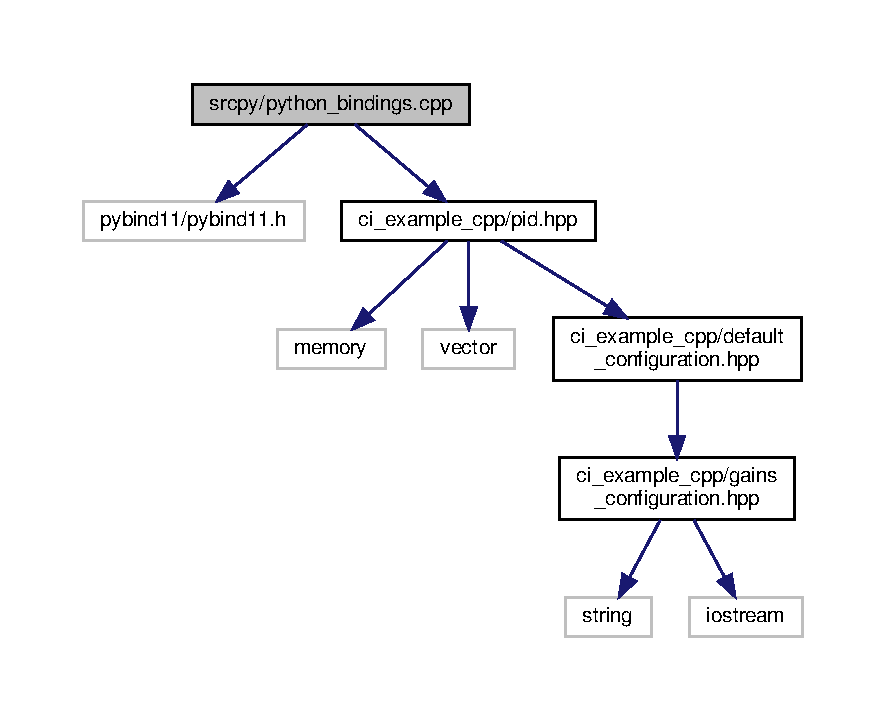
\includegraphics[width=350pt]{python__bindings_8cpp__incl}
\end{center}
\end{figure}
\subsection*{Functions}
\begin{DoxyCompactItemize}
\item 
\mbox{\Hypertarget{python__bindings_8cpp_a9665291aa25282deadab758bb4c20dd7}\label{python__bindings_8cpp_a9665291aa25282deadab758bb4c20dd7}} 
{\bfseries P\+Y\+B\+I\+N\+D11\+\_\+\+M\+O\+D\+U\+LE} (basic\+\_\+pid, m)
\end{DoxyCompactItemize}


\subsection{Detailed Description}
license License B\+S\+D-\/3-\/\+Clause 

\begin{DoxyCopyright}{Copyright}
Copyright (c) 2019, New York University and Max Planck Gesellschaft. 
\end{DoxyCopyright}

\chapter{Example Documentation}
\hypertarget{demo_pid_8cpp-example}{}\section{demo\+\_\+pid.\+cpp}
Create the default P\+ID controller and compute the control once. This illustrates in the simplest way the use of the P\+ID class A\+PI.


\begin{DoxyCodeInclude}

\textcolor{preprocessor}{#include "\hyperlink{pid_8hpp}{ci\_example\_cpp/pid.hpp}"} 

\textcolor{keywordtype}{void} \hyperlink{demo__pid_8cpp_aa5343637e5c7a19c19aae1beed976ab6}{run\_demo}()\{

  \textcolor{comment}{// PID controller with default gains values}
  \hyperlink{classci__example__cpp_1_1PID}{ci\_example\_cpp::PID}& controller = 
      \hyperlink{pid_8hpp_ae98dfa6f474e368f3d1865d65406ec1f}{ci\_example\_cpp::get\_default\_pid}();
  
  \textcolor{comment}{// example of force computation}
  \textcolor{keywordtype}{double} current\_position=1;
  \textcolor{keywordtype}{double} current\_velocity=1;
  \textcolor{keywordtype}{double} delta\_time=0.01;
  \textcolor{keywordtype}{double} target\_position=2;
  \textcolor{keywordtype}{double} force = controller.\hyperlink{classci__example__cpp_1_1PID_a75a4ccf0455e48e84af23e1d28b0337d}{compute}(current\_position,
                    current\_velocity,
                    target\_position,
                    delta\_time);
  std::cout<< \textcolor{stringliteral}{"computed force: "} << force << std::endl;

  \textcolor{comment}{// resetting integral of the controller}
  \textcolor{comment}{// (useless here because we do not reuse it)}
  controller.\hyperlink{classci__example__cpp_1_1PID_a65d98fccd38cc385debc3d15670caf0e}{reset\_integral}();
  
\}


\textcolor{keywordtype}{int} \hyperlink{demo__pid_8cpp_ae66f6b31b5ad750f1fe042a706a4e3d4}{main}()\{
  
  \textcolor{keywordflow}{try} \{
    \hyperlink{demo__pid_8cpp_aa5343637e5c7a19c19aae1beed976ab6}{run\_demo}();
  \} \textcolor{keywordflow}{catch}(\textcolor{keyword}{const} std::exception& e)\{
    std::cout << \textcolor{stringliteral}{"demo failed !\(\backslash\)nerror message:\(\backslash\)n"} << e.what() << std::endl;
    \textcolor{keywordflow}{return} 1; \textcolor{comment}{// informs continuous integration that this demo did not run successfully}
  \}

  \textcolor{keywordflow}{return} 0; \textcolor{comment}{// informs continuous integration that this demo did run successfully}

\}
\end{DoxyCodeInclude}
 
\hypertarget{demo_pid_load_from_file_8cpp-example}{}\section{demo\+\_\+pid\+\_\+load\+\_\+from\+\_\+file.\+cpp}
Load the P\+ID gains from a yaml file and create a P\+ID controller from them.\+This illustrates how to safely use the A\+PI when yaml file parsing is wanted.


\begin{DoxyCodeInclude}

\textcolor{preprocessor}{#include "\hyperlink{pid_8hpp}{ci\_example\_cpp/pid.hpp}"}
\textcolor{preprocessor}{#include "\hyperlink{file__configuration_8hpp}{ci\_example\_cpp/file\_configuration.hpp}"} 
\textcolor{preprocessor}{#include <stdexcept>}

\textcolor{keywordtype}{void} \hyperlink{demo__pid__load__from__file_8cpp_aa5343637e5c7a19c19aae1beed976ab6}{run\_demo}()\{

  \textcolor{comment}{/* displaying what this demo is about */}
  std::cout << 
    \textcolor{stringliteral}{"This demo shows how to create an executable run by the continuous integration\(\backslash\)n"} <<
    \textcolor{stringliteral}{"which depends on a configuration file. In the solution showed here, the absolute path\(\backslash\)n"} <<
    \textcolor{stringliteral}{"to the configuration file is set during pre-compilation. See code in
       /demos/demo\_pid\_load\_from\_file.cpp\(\backslash\)n"} <<
    \textcolor{stringliteral}{"for details\(\backslash\)n\(\backslash\)n"};
  
  \textcolor{comment}{/* reading gains (kp,kd,ki) from yaml config */}

  \textcolor{comment}{// (look at the CMakeLists.txt to see why TEST\_PID\_GAINS\_YAML\_FILE\_PATH is replaced by correct abs path 
       during compilation)}
  std::string config\_file\_path = TEST\_PID\_GAINS\_YAML\_FILE\_PATH;

  \textcolor{comment}{// Gains\_configuration is the base class for all configuration, including}
  \textcolor{comment}{// the one read from yaml file, as done here. }
  \hyperlink{classci__example__cpp_1_1File__configuration}{ci\_example\_cpp::File\_configuration} gains = 
      \hyperlink{classci__example__cpp_1_1File__configuration}{ci\_example\_cpp::File\_configuration}(config\_file\_path);

  \textcolor{comment}{// printing to standard output the gains}
  std::cout << \textcolor{stringliteral}{"gains read from configuration file:"} << std::endl;
  \hyperlink{gains__configuration_8hpp_a2400ff05e31dee6aced75d9c230b9fe5}{ci\_example\_cpp::print\_configuration}(gains);

  \textcolor{comment}{// checking reading the config file when fine}
  \textcolor{comment}{// if not, throwing corresponding error}
  \textcolor{keywordflow}{if} (gains.\hyperlink{classci__example__cpp_1_1File__configuration_aa3cae137be3b59e61d13c2a9b1ec8b6a}{has\_error}())\{
    \textcolor{keywordflow}{throw} std::runtime\_error(gains.\hyperlink{classci__example__cpp_1_1File__configuration_aaf67f7d61d467563a4dce8aa69306a6a}{get\_error}());
  \}

  \textcolor{comment}{/* creating and running the controller */}

  \textcolor{comment}{// PID controller creation}
  \hyperlink{classci__example__cpp_1_1PID}{ci\_example\_cpp::PID} controller(gains);
  
  \textcolor{comment}{// example of force computation}
  \textcolor{keywordtype}{double} current\_position=1;
  \textcolor{keywordtype}{double} current\_velocity=1;
  \textcolor{keywordtype}{double} delta\_time=0.01;
  \textcolor{keywordtype}{double} target\_position=2;
  \textcolor{keywordtype}{double} force = controller.compute(current\_position,current\_velocity,target\_position,delta\_time);
  std::cout<< \textcolor{stringliteral}{"computed force: "} << force << std::endl;

  \textcolor{comment}{// resetting integral of the controller}
  controller.reset\_integral();
  
\}

\textcolor{keywordtype}{int} \hyperlink{demo__pid__load__from__file_8cpp_ae66f6b31b5ad750f1fe042a706a4e3d4}{main}()\{
  
  \textcolor{keywordflow}{try} \{
    \hyperlink{demo__pid__load__from__file_8cpp_aa5343637e5c7a19c19aae1beed976ab6}{run\_demo}();
  \} \textcolor{keywordflow}{catch}(\textcolor{keyword}{const} std::runtime\_error& e)\{
    std::cout << \textcolor{stringliteral}{"demo failed !\(\backslash\)nerror message:\(\backslash\)n"} << e.what() << std::endl;
    \textcolor{keywordflow}{return} 1; \textcolor{comment}{// informs continuous integration that this demo did not run successfully}
  \}

  \textcolor{keywordflow}{return} 0; \textcolor{comment}{// informs continuous integration that this demo did run successfully}

\}
\end{DoxyCodeInclude}
 
%--- End generated contents ---

% Index
\backmatter
\newpage
\phantomsection
\clearemptydoublepage
\addcontentsline{toc}{chapter}{Index}
\printindex

\end{document}
